\newtheorem{theorem}{定理}
\newtheorem{proposition}{命题}

\chapter{引论}

这一章首先给出下面就要研究的那些概念的定义，譬如什么是常微分方程组，什么叫作它的解，以及存在多少这种解；这样一些主要问题都要在本章中得到回答。解的数量由一些存在和唯一性定理来确定。本章只叙述这些定理而不加以证明；它们的证明原来安排在第四章。到了那里，这些定理在本章中已经被多次使用，读者也就更容易看清它们的作用和意义。除了这些基本知识以外，本章还要介绍几种最简单类型微分方程的解法。本章最后讨论复值函数的微分方程以及它们的复值解，并介绍线性微分方程组的最基本性质。

\section*{记号与约定}
\addcontentsline{toc}{section}{记号与约定}

许多物理问题中的自变量是时间，因此本章通常用实数 \(t\) 表示自变量，并把它限制在开区间
\[
 I=(r_1,r_2)\subseteq\R,
\qquad -\infty\le r_1<r_2\le+\infty
\]
上。端点可以取无穷。标量未知函数通常记为 \(y:I\to\R\)。一般的一阶导数写成 \(y'\)，高阶导数写成 \(y^{(k)}\)，并约定 \(y^{(0)}=y\)。在力学或控制论语境中，为提示“对时间求导”，也会使用牛顿记号 \(\dot y,\ddot y\)；本章始终把
\[
 \dot y=y',\qquad \ddot y=y''
\]
理解为同一个运算，不另立一套含义。

当有 \(n\) 个未知函数时，把它们排成列向量
\begin{equation}
 \vect{x}(t)=
 \begin{pmatrix}
  x_1(t)\\
  x_2(t)\\
  \vdots\\
  x_n(t)
 \end{pmatrix}
 \in\mathbb F^n,
 \qquad \mathbb F=\R\ \text{或}\ \C.
 \label{eq:ch1-state-vector}
\end{equation}
原书使用上标 \(x^1,\ldots,x^n\)；为了避免与幂混淆，本稿统一使用下标 \(x_1,\ldots,x_n\)。一阶显式系统统一写成
\begin{equation}
 \vect{x}'=\vect{f}(t,\vect{x}),
 \qquad
 \vect{f}:\Omega\subseteq\R\times\R^n\longrightarrow\R^n,
 \label{eq:ch1-general-system}
\end{equation}
其中
\[
 \vect{f}(t,\vect{x})=
 \begin{pmatrix}
  f_1(t,x_1,\ldots,x_n)\\
  \vdots\\
  f_n(t,x_1,\ldots,x_n)
 \end{pmatrix}.
\]
如果 \(\vect{f}\) 对状态变量可微，则记
\[
 D_{\vect{x}}\vect{f}(t,\vect{x})
 =
 \begin{pmatrix}
  \dfrac{\partial f_1}{\partial x_1}(t,\vect{x})&\cdots&
  \dfrac{\partial f_1}{\partial x_n}(t,\vect{x})\\
  \vdots&\ddots&\vdots\\
  \dfrac{\partial f_n}{\partial x_1}(t,\vect{x})&\cdots&
  \dfrac{\partial f_n}{\partial x_n}(t,\vect{x})
 \end{pmatrix}
 \in\mathbb F^{n\times n}.
\]
矩阵总是从左边作用于列向量。线性系统的标准形式写作
\[
 \vect{x}'=\mat{A}(t)\vect{x}+\vect{b}(t),
\]
其中 \(\mat{A}(t)\in\mathbb F^{n\times n}\)，\(\vect{b}(t)\in\mathbb F^n\)。符号 \(\vect{x}\) 表示整条解函数，符号 \(\vect{x}(t)\) 表示它在时刻 \(t\) 的状态；两者不能混同。除 §5 明确讨论复值时，本章默认 \(\mathbb F=\R\)。

\section{一阶微分方程}

微分方程是指这样的方程：其中未知的是一个或多个函数，而且方程中不仅含有函数本身，还含有它们的导函数。如果未知函数依赖于多个自变量，并出现偏导数，那么称这类方程为偏微分方程。如果未知函数只依赖于一个自变量，那么称这类方程为常微分方程。今后只讨论常微分方程。

一般的一阶标量微分方程可以写成
\begin{equation}
 F(t,y,y')=0.
 \label{eq:ch1-first-order-implicit}
\end{equation}
这里 \(t\) 是自变量，\(y\) 是 \(t\) 的未知函数，\(y'\) 是未知函数的导数，而 \(F\) 是三个给定变量的函数。函数 \(F\) 未必对所有三元组都有定义，因此需要考虑它的定义域 \(B\subseteq\R^3\)。\(B\) 中的点用坐标
\[
 (t,y,y')
\]
表示。

设 \(y=\varphi(t)\) 在区间 \(r_1<t<r_2\) 上有定义，其中不排除 \(r_1=-\infty\) 或 \(r_2=+\infty\) 的情形。如果：
\begin{enumerate}[label=\arabic*.]
 \item \(\varphi\) 在整个区间上具有一阶导数，特别地连续；
 \item 对每个 \(t\in(r_1,r_2)\)，点 \((t,\varphi(t),\varphi'(t))\) 都属于定义域 \(B\)；
 \item 用 \(\varphi(t)\) 和 \(\varphi'(t)\) 替换上式中的 \(y\) 与 \(y'\) 后，
 \[
  F(t,\varphi(t),\varphi'(t))=0
 \]
 在整个区间上恒成立，
\end{enumerate}
那么就称 \(y=\varphi(t)\) 是微分方程 \eqref{eq:ch1-first-order-implicit} 的解，并称 \((r_1,r_2)\) 是这个解的定义区间。必须把“函数在区间内满足方程”和“函数图形始终落在 \(F\) 的定义域中”同时记住；方程本身不能在一个没有定义的点上成立。

关系式 \eqref{eq:ch1-first-order-implicit} 联系着三个变量 \(t,y,y'\)。在某些情形下，它可以唯一地解出 \(y'\)，于是得到一个形如
\begin{equation}
 y'=f(t,y)
 \label{eq:ch1-first-order-explicit}
\end{equation}
的方程。这样的方程称为已解出导数的一阶微分方程。与隐式形式相比，显式形式通常更容易研究。以下不总把 \eqref{eq:ch1-first-order-explicit} 看成从 \eqref{eq:ch1-first-order-implicit} 解出的特殊结果，而是直接把 \(f\) 当作给定的二元函数。

为了作几何解释，在平面 \(P\) 中取横轴为 \(t\)，纵轴为 \(y\)。函数 \(f\) 可能只在 \(P\) 的某个集合 \(\Gamma\) 上有定义，而不一定在整个平面上有定义，如图~\ref{fig:ch1-domain} 所示。以后总假设 \(\Gamma\) 是开集：对每个 \(p\in\Gamma\)，存在以 \(p\) 为中心、半径为正的圆盘完全含于 \(\Gamma\) 中。还假设 \(f\) 以及偏导数
\[
 \frac{\partial f}{\partial y}
\]
都在 \(\Gamma\) 上连续。

若 \(y=\varphi(t)\) 是 \eqref{eq:ch1-first-order-explicit} 的解，那么它的图形就是平面 \(P\) 中由 \(y=\varphi(t)\) 表示的曲线。因为 \(y'\) 在区间上存在，所以曲线处处有切线；因为函数值落在 \(f\) 的定义域中，所以整条曲线都在 \(\Gamma\) 内。这条曲线称为微分方程的积分曲线。

\begin{figure}[H]
 \centering
 \resizebox{0.52\textwidth}{!}{\begin{tikzpicture}[
    x=0.85cm,y=0.85cm,
    >=Stealth,
    line cap=round,
    line join=round,
    axis/.style={->,thin},
    boundary/.style={thick},
    integral/.style={thin},
    every node/.style={font=\small}
]
  % Define the domain boundary once, then reuse it for drawing and clipping.
  \def\GammaPath{
    (-0.85,1.15)
    .. controls (-1.05,1.65) and (-0.75,2.35) .. (-0.20,2.65)
    .. controls (0.65,3.15) and (2.10,3.25) .. (2.75,2.85)
    .. controls (3.35,2.45) and (3.70,1.75) .. (3.90,1.10)
    .. controls (4.05,0.60) and (3.70,0.35) .. (3.15,0.30)
    .. controls (2.45,0.20) and (1.70,0.30) .. (1.10,0.55)
    .. controls (0.55,0.80) and (0.15,0.95) .. (-0.35,0.90)
    .. controls (-0.65,0.88) and (-0.82,1.00) .. (-0.85,1.15)
    -- cycle
  }
  % Coordinate axes.
  \draw[axis] (-1.1,0)--(4.7,0) node[right] {$t$};
  \draw[axis] (0,-0.75)--(0,3.55) node[above] {$y$};
  \node[below left=1pt] at (0,0) {$O$};

  % Clip all integral curves to the open domain Gamma.
  \begin{scope}
    \clip \GammaPath;
    \draw[integral] (-1.15,1.30).. controls (-0.45,2.15) and (0.90,2.72)..(2.65,3.02);
    \draw[integral] (-1.05,1.18).. controls (-0.35,1.98) and (1.05,2.45)..(3.00,2.75);
    \draw[integral] (-1.00,1.05).. controls (-0.20,1.75) and (1.20,2.15)..(3.30,2.48);
    \draw[integral] (-0.85,0.95).. controls (0.10,1.48) and (1.55,1.88)..(3.55,2.15);
    \draw[integral] (-0.70,0.85).. controls (0.35,1.25) and (1.95,1.55)..(3.85,1.78);
    \draw[integral,very thick] (-0.55,0.75).. controls (0.60,1.00) and (2.15,1.20)..(4.05,1.48);
    \draw[integral] (-0.35,0.65).. controls (0.75,0.72) and (2.25,0.90)..(4.05,1.15);
    \draw[integral] (-0.15,0.55).. controls (0.90,0.45) and (2.30,0.60)..(4.00,0.85);
    \draw[integral] (0.15,0.45).. controls (1.10,0.15) and (2.45,0.10)..(3.75,0.48);
  \end{scope}

  % Redraw the smooth boundary above the clipped curves.
  \draw[boundary] \GammaPath;
  \fill (0.75,0.97) circle (1.7pt);
  \node[below left=1pt] at (0.75,0.97) {$p$};
  \node[rotate=8,font=\footnotesize] at (2.15,1.43) {$y=\varphi(t)$};
  \node at (2.95,2.24) {$\Gamma$};
\end{tikzpicture}
}
 \caption{开区域 \(\Gamma\)、方向场以及过点 \(p\) 的积分曲线（原书图 1）。}
 \label{fig:ch1-domain}
\end{figure}

\subsection{存在和唯一性定理}

正如代数学中回答代数方程根的个数问题的定理十分重要一样，微分方程理论中关于解的存在与唯一性的问题也是基本的理论问题。例如，代数基本定理断言：一个 \(n\) 次多项式在复数域中恰有 \(n\) 个根，重根按重数计算。微分方程的情形则不同：一个微分方程通常有无限多个解。因此，对微分方程不应先问“有几个解”，而应问怎样描述给定方程的全部解。本节的定理 1 回答这个问题，而原书把它的证明放在第四章 §20；本翻新稿把证明统一移到\hyperref[sec:existence-proofs]{本章补证}。

\begin{theorem}[一阶标量方程的存在唯一性]
 \label{thm:ch1-scalar-existence}
 设函数 \(f(t,y)\) 在 \((t,y)\) 平面的某个开集 \(\Gamma\) 上有定义，并且 \(f\) 及其偏导数 \(\partial f/\partial y\) 都在整个 \(\Gamma\) 上连续。考虑
 \[
  y'=f(t,y).
 \]
 则有以下两条结论。
 \begin{enumerate}[label=\arabic*.]
  \item 对 \(\Gamma\) 中任意一点 \((t_0,y_0)\)，存在一个包含 \(t_0\) 的区间，以及定义在该区间上的解 \(y=\varphi(t)\)，满足
  \[
   \varphi(t_0)=y_0.
  \]
  \item 如果 \(y=\varphi(t)\) 和 \(y=\chi(t)\) 是同一方程的两个解，并且它们在某个共同时刻 \(t_0\) 相等，即
  \[
   \varphi(t_0)=\chi(t_0),
  \]
  那么对两者都有定义的每个 \(t\)，必有 \(\varphi(t)=\chi(t)\)。
 \end{enumerate}
\end{theorem}

证明见\hyperref[sec:existence-proofs]{本章补证}。其中“局部构造”和“公共区间上的唯一性”两小节，在 \(n=1\) 时正是定理~\ref{thm:ch1-scalar-existence} 的证明；“最大解的存在与唯一”一节则证明定理第二条可以进一步组织为最大延拓的结论。原证明路线是 Picard 逐次逼近：先把微分方程改写成积分方程，再在足够小的时间区间上作压缩映射。

数 \(t_0\) 称为解的初始时刻，\(y_0\) 称为初始值，关系式 \(y(t_0)=y_0\) 称为初始条件。也说解 \(y=\varphi(t)\) 满足这个初始条件，或具有这个初始值。当说一个解满足初始条件时，总默认它的定义区间包含 \(t_0\)。于是定理 1 的第一条断言：\(\Gamma\) 中每一点的坐标都可以作为某个解的初始值；第二条断言：具有相同初始值的两个解，在共同定义区间上完全相同。

定理 1 的几何含义是：通过 \(\Gamma\) 中每一点 \((t_0,y_0)\)，有且只有一条积分曲线。这里必须仔细理解“有且只有一条”。即使允许某个方程在某一点附近拥有两个具有相同初始值、但定义区间不同的解，定理仍只断言它们在共同区间上相等。它没有断言两个解原有的定义区间必须相同。

如果两个解的定义区间分别为 \(I=(r_1,r_2)\) 和 \(J=(s_1,s_2)\)，且
\[
 s_1\le r_1<r_2\le s_2,
\]
并且定义在 \(J\) 上的解限制到 \(I\) 后等于原来定义在 \(I\) 上的解，那么称 \(J\) 上的解是 \(I\) 上解的延拓。注意力自然集中在不能再向左或向右延拓的解上；这种解称为不可延拓解，或最大解。

在定理 1 的条件下，每一个解都可以用唯一的方法延拓到不可延拓解。这个命题在\hyperref[sec:existence-proofs]{本章补证}的“最大解的存在与唯一”一节中明确证明。把每个解都换成其唯一的不可延拓延拓后，“过每一点恰有一条积分曲线”的几何陈述就没有歧义了。

\subsection{方向场与例题}

积分曲线给出方程单个解的几何解释；方程本身还可以用方向场解释。对 \(\Gamma\) 的每一点 \((t,y)\)，取一条斜率为 \(f(t,y)\) 的直线；所有这些直线组成对应于方程的平面方向场。因为积分曲线在点 \((t,\varphi(t))\) 处的斜率为
\[
 \varphi'(t)=f(t,\varphi(t)),
\]
所以任一积分曲线在每一点都与该点的方向场直线相切。这就是方程的几何解释与解的几何解释之间的联系，如图~\ref{fig:ch1-direction-field} 所示。

\begin{figure}[H]
 \centering
 \resizebox{0.46\textwidth}{!}{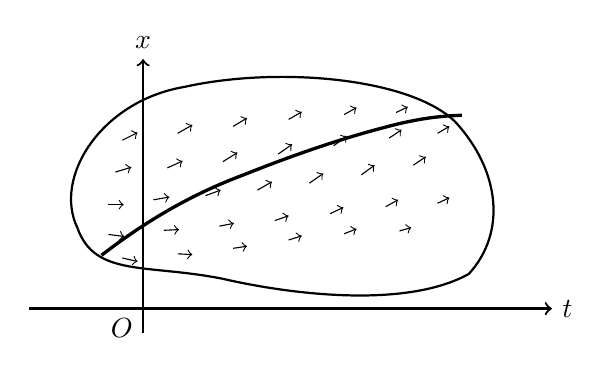
\begin{tikzpicture}[x=0.88cm,y=0.88cm,thick]
  \draw[thick] (-3.1,-0.38) .. controls (-3.45,0.35) and (-2.75,1.45) .. (-1.55,1.65)
    .. controls (-0.2,1.95) and (1.7,1.78) .. (2.35,1.15)
    .. controls (3.0,0.45) and (3.1,-0.45) .. (2.55,-1.05)
    .. controls (1.65,-1.55) and (0.0,-1.35) .. (-1.0,-1.12)
    .. controls (-2.1,-0.9) and (-2.85,-1.1) .. (-3.1,-0.38);
  \draw[->] (-3.8,-1.55)--(3.75,-1.55) node[right] {$t$};
  \draw[->] (-2.15,-1.9)--(-2.15,2.05) node[above] {$x$};
  \node[below left] at (-2.15,-1.55) {$O$};
  % A sampled direction field; each small segment has slope depending on t and x.
  \foreach \x/\y/\dx/\dy in {
  -2.65/-0.05/0.22/0.00,-2.0/0.02/0.23/0.04,-1.25/0.08/0.22/0.08,-0.5/0.16/0.21/0.12,0.25/0.26/0.20/0.14,1.0/0.38/0.19/0.14,1.75/0.52/0.18/0.12,
  -2.55/0.42/0.23/0.07,-1.8/0.48/0.22/0.10,-1.0/0.57/0.21/0.13,-0.2/0.68/0.20/0.14,0.6/0.80/0.19/0.14,1.4/0.91/0.18/0.12,2.1/0.98/0.17/0.10,
  -2.45/0.88/0.22/0.11,-1.65/0.98/0.21/0.12,-0.85/1.08/0.20/0.12,-0.05/1.18/0.19/0.11,0.75/1.25/0.18/0.10,1.5/1.28/0.17/0.08,
  -2.65/-0.48/0.23/-0.03,-1.85/-0.42/0.22/0.01,-1.05/-0.36/0.21/0.04,-0.25/-0.28/0.20/0.07,0.55/-0.18/0.19/0.09,1.35/-0.08/0.18/0.10,2.1/-0.03/0.17/0.08,
  -2.45/-0.82/0.22/-0.05,-1.65/-0.76/0.21/-0.01,-0.85/-0.68/0.20/0.03,-0.05/-0.56/0.19/0.06,0.75/-0.47/0.18/0.07,1.55/-0.43/0.17/0.05}
    {\draw[->,thin] (\x,\y)--++(\dx,\dy);}
  \draw[very thick] (-2.75,-0.78) .. controls (-2.1,-0.28) and (-1.45,0.1) .. (-0.7,0.38)
    .. controls (0.1,0.7) and (0.85,0.95) .. (1.55,1.12)
    .. controls (1.9,1.2) and (2.15,1.23) .. (2.45,1.24);
\end{tikzpicture}
}
 \caption{实心点表示取样点 \((t,y)\)，以该点为中点的短线段表示斜率 \(f(t,y)\)；粗实线为一条积分曲线，在其上的取样点处与对应短线段相切（原书图 2）。}
 \label{fig:ch1-direction-field}
\end{figure}

\paragraph{例 1：指数增长与衰减.}
为了说明定理 1，特别是它的唯一性部分的含义，求解
\begin{equation}
 y'=ay,
 \label{eq:ch1-exponential}
\end{equation}
其中 \(a\in\R\)。这里
\[
 f(t,y)=ay,\qquad \frac{\partial f}{\partial y}=a.
\]
函数实际上只依赖于 \(y\)，定义集合可以取整个平面 \(P\)。函数 \(f\) 及其偏导数在整个平面上连续，因此定理 1 适用。直接代入可知，对任意常数 \(c\in\R\)，
\begin{equation}
 y(t)=ce^{at}
 \label{eq:ch1-exponential-solutions}
\end{equation}
都是 \eqref{eq:ch1-exponential} 的解，并且都定义在整个实轴 \(-\infty<t<+\infty\) 上，所以是不可延拓解。

还要证明 \eqref{eq:ch1-exponential-solutions} 给出了全部解。设 \(y=\varphi(t)\) 是任一解，在它的定义区间中取一点 \(t_0\)，记 \(y_0=\varphi(t_0)\)。取
\[
 c=y_0e^{-at_0}.
\]
那么解 \(ce^{at}\) 与 \(\varphi(t)\) 具有相同的初始值 \((t_0,y_0)\)。由定理 1 的第二部分，它们在共同区间上相同。因此，随着 \(c\) 取遍一切实数，公式 \eqref{eq:ch1-exponential-solutions} 确实给出全部解。

\paragraph{例 2：放射性衰变.}
用 \(y(t)\) 表示到时刻 \(t\) 尚未衰变的放射性物质量。由物理上的假设，若不能追踪整个反应过程，至少可以说衰变速度与剩余物质量成正比：
\begin{equation}
 y'(t)=-\beta y(t),
 \label{eq:ch1-radioactive}
\end{equation}
其中 \(\beta>0\) 是依赖于物质性质的常数，负号表示物质量在减少。这个方程正是例 1 中 \(a=-\beta\) 的情形，所以
\[
 y(t)=ce^{-\beta t}.
\]
若已知在 \(t=0\) 时物质量为 \(y_0\)，则 \(c=y_0\)，于是
\[
 y(t)=y_0e^{-\beta t}.
\]
这里的 \(\beta\) 具有量纲 \(1/\text{秒}\)。通常用半衰期代替 \(\beta\) 描述衰变快慢。半衰期 \(T\) 是物质量减到原来一半所需的时间，因此
\[
 \frac{y_0}{2}=y_0e^{-\beta T}.
\]
当 \(y_0>0\) 时约去 \(y_0\)，得到
\[
 e^{-\beta T}=\frac12,
 \qquad
 T=\frac{\ln 2}{\beta}.
\]

\section{一些初等的求积方法}

研究微分方程时，首先遇到的通常是如何求解的问题。这与代数学中的情况类似。代数学曾试图用开根给出任意次方程的解：二次方程有求根公式，三次方程有 Cardan 公式，四次方程有 Ferrari 公式；后来证明，用根式给出四次以上方程的一般公式是不可能的。可是，始终可以求数值系数方程的近似解，也可以研究方程的根如何依赖系数。

微分方程理论早期也力图用初等函数以及这些函数的积分把解表示出来，即所谓“用求积方式积分出微分方程”。当人们弄清只有少数类型的方程才具有这种意义下的解以后，理论重点便转移到研究解的一般性质和变化规律。本节只介绍几类最简单的一阶方程，它们仍展示了“积分—隐式解—分支—唯一性”之间的关系。

\subsection{正合方程}

\textbf{(A) 正合方程.} 考虑
\begin{equation}
 y'=\frac{g(t,y)}{h(t,y)}.
 \label{eq:ch1-exact-normal}
\end{equation}
假设 \(g,h\) 在 \((t,y)\) 平面的某个开集 \(\Gamma\) 上有定义且连续；分母 \(h(t,y)\) 在 \(\Gamma\) 的每一点都不为零。再假设微分形式
\[
 h(t,y)\,\dd y-g(t,y)\,\dd t
\]
在整个 \(\Gamma\) 上是全微分。这意味着存在函数 \(F:\Gamma\to\R\)，使得
\begin{equation}
 \frac{\partial F}{\partial y}(t,y)=h(t,y),
 \qquad
 \frac{\partial F}{\partial t}(t,y)=-g(t,y).
 \label{eq:ch1-exact-potential}
\end{equation}
于是 \eqref{eq:ch1-exact-normal} 可以约定地写成
\[
 h(t,y)\,\dd y-g(t,y)\,\dd t=0,
\]
而左边正是 \(\dd F\)。

\begin{proposition}[正合方程的解]
 \label{prop:ch1-exact}
 在以上条件下，方程 \eqref{eq:ch1-exact-normal} 的每一个解 \(y=\varphi(t)\) 都满足
 \[
  F(t,\varphi(t))=\text{常数}.
 \]
 反之，由含任意常数 \(c\) 的隐式关系
 \begin{equation}
  F(t,y)=c
  \label{eq:ch1-exact-integral}
 \end{equation}
 在某个区间上确定的可微函数 \(y=\varphi(t)\)，都是方程 \eqref{eq:ch1-exact-normal} 的解。
\end{proposition}

\begin{proof}
先设 \(y=\varphi(t)\) 是 \eqref{eq:ch1-exact-normal} 在区间 \(r_1<t<r_2\) 上的解。对这个区间中的每个 \(t\)，都有
\[
 h(t,\varphi(t))\varphi'(t)-g(t,\varphi(t))=0.
\]
由 \eqref{eq:ch1-exact-potential}，左边正是 \(F(t,\varphi(t))\) 对 \(t\) 的全导数：
\[
 \frac{\dd}{\dd t}F(t,\varphi(t))
 =F_t(t,\varphi(t))+F_y(t,\varphi(t))\varphi'(t)
 =-g(t,\varphi(t))+h(t,\varphi(t))\varphi'(t)=0.
\]
根据微积分中的已知结论，在连通区间上导数为零的函数为常数，所以 \(F(t,\varphi(t))\) 在整个定义区间上为常数。

反过来，若 \(y=\varphi(t)\) 是由 \eqref{eq:ch1-exact-integral} 定义的解，即 \(F(t,\varphi(t))\equiv c\)，对 \(t\) 求导，得到
\[
 F_t(t,\varphi(t))+F_y(t,\varphi(t))\varphi'(t)=0.
\]
代入 \eqref{eq:ch1-exact-potential}，便有
\[
 h(t,\varphi(t))\varphi'(t)-g(t,\varphi(t))=0.
\]
因为 \(h\neq0\)，这正是 \eqref{eq:ch1-exact-normal}。命题得证。
\end{proof}

几何上，方程 \eqref{eq:ch1-exact-normal} 的每一条积分曲线都完全位于函数 \(F(t,y)\) 的某条水平线
\[
 F(t,y)=c
\]
上。反过来，每一条水平线的连通部分，只要能够表示为某个区间上的函数 \(y=\varphi(t)\)，就是积分曲线。可是，水平线可能由分开的几段组成；在这种情况下，一个常数 \(c\) 可能确定几条不同的积分曲线。换言之，同一个隐式公式可能对应几个，甚至无限多个，不可延拓解。例 3 将具体展示这一点。

\subsection{一阶线性方程}

\textbf{(B) 线性方程.} 求解
\begin{equation}
 y'=a(t)y+b(t),
 \label{eq:ch1-linear-scalar}
\end{equation}
其中 \(a(t),b(t)\) 在区间
\[
 I=(r_1,r_2)
\]
上有定义且连续，端点可以取无穷。此时
\[
 \Gamma=I\times\R.
\]
若两个端点都有限，则 \(\Gamma\) 是带形区域；若只有一个端点有限，则它是半平面；若两个端点为无穷，则 \(\Gamma\) 是整个平面。在整个 \(\Gamma\) 上，方程右端及其对 \(y\) 的偏导数都连续，所以定理 1 的条件满足。

固定 \(t_0\in I\)，记
\begin{equation}
 A(t)=\int_{t_0}^{t}a(s)\,\dd s.
 \label{eq:ch1-linear-integrated-coefficient}
\end{equation}
函数 \(A(t)\) 在整个 \(I\) 上有定义。方程 \eqref{eq:ch1-linear-scalar} 的全部解可写成
\begin{equation}
 y(t)=e^{A(t)}
 \left(
  c+\int_{t_0}^{t}e^{-A(s)}b(s)\,\dd s
 \right),
 \qquad c\in\R.
 \label{eq:ch1-linear-solution}
\end{equation}
这些解都在整个 \(I\) 上有定义，因而是相对于给定定义域 \(I\times\R\) 的不可延拓解：在区间端点之外，方程右端本来就没有定义。

\begin{proof}[公式 \eqref{eq:ch1-linear-solution} 的验证与完整性]
先验证这些函数确实是解。由微积分基本定理，
\[
 \frac{\dd}{\dd t}e^{A(t)}=a(t)e^{A(t)},
 \qquad
 \frac{\dd}{\dd t}\int_{t_0}^{t}e^{-A(s)}b(s)\,\dd s
 =e^{-A(t)}b(t).
\]
因此
\[
 \begin{aligned}
  y'(t)
  &=a(t)e^{A(t)}
    \left(c+\int_{t_0}^{t}e^{-A(s)}b(s)\,\dd s\right)
    +e^{A(t)}e^{-A(t)}b(t)\\
  &=a(t)y(t)+b(t).
 \end{aligned}
\]

现在证明公式包含全部解。设 \(y=\varphi(t)\) 是 \eqref{eq:ch1-linear-scalar} 在某个区间 \(J\subseteq I\) 上的任意解，取 \(\tau_0\in J\)，令 \(\xi_0=\varphi(\tau_0)\)。需要选择常数 \(c\)，使公式给出的解在 \(\tau_0\) 处等于 \(\xi_0\)。条件为
\[
 \left(
  c+\int_{t_0}^{\tau_0}e^{-A(s)}b(s)\,\dd s
 \right)e^{A(\tau_0)}
 =\xi_0.
\]
这是关于 \(c\) 的一次方程，而且未知量 \(c\) 的系数 \(e^{A(\tau_0)}\) 不为零，所以可唯一地解出
\[
 c=\xi_0e^{-A(\tau_0)}
 -\int_{t_0}^{\tau_0}e^{-A(s)}b(s)\,\dd s.
\]
由定理 1 的唯一性，公式给出的解与 \(\varphi\) 在共同定义区间上完全相同。因此公式 \eqref{eq:ch1-linear-solution} 包含全部解。
\end{proof}

为了与教科书中常见的记忆方法对照，可以重新推导这个公式。先考虑齐次方程
\begin{equation}
 y'=a(t)y.
 \label{eq:ch1-linear-homogeneous}
\end{equation}
在 \(y\neq0\) 时，把它写成
\[
 \frac{\dd y}{y}-a(t)\,\dd t=0.
\]
这是正合方程。取
\[
 F(t,y)=\ln|y|-A(t),
\]
则齐次解由
\[
 \ln|y|-A(t)=c_1
\]
确定，即
\begin{equation}
 y=ce^{A(t)}.
 \label{eq:ch1-linear-homogeneous-solution}
\end{equation}
这里 \(c\) 可以取任意实数；\(y=0\) 对应 \(c=0\)。严格地说，先除以 \(y\) 的推导没有覆盖 \(y=0\)，但这个遗漏可以由公式的完整性证明，或由 \(c=0\) 补上，因此不影响齐次解公式。

再用常数变易法求非齐次解。设
\[
 y=c(t)e^{A(t)},
\]
其中 \(c(t)\) 是待定函数。代入 \eqref{eq:ch1-linear-scalar}，得到
\[
 c'(t)e^{A(t)}+c(t)a(t)e^{A(t)}
 =a(t)c(t)e^{A(t)}+b(t).
\]
含有 \(a(t)\) 的项相消，于是
\[
 c'(t)e^{A(t)}=b(t),
 \qquad
 c(t)=c_0+\int_{t_0}^{t}e^{-A(s)}b(s)\,\dd s.
\]
代回即得 \eqref{eq:ch1-linear-solution}。这就是常数变易法：把齐次解中的常数换成时间函数。

\subsection{例题}

\paragraph{例 1：可分离变量方程.}
求解
\begin{equation}
 y'=f(t)g(y).
 \label{eq:ch1-separable}
\end{equation}
假设 \(f(t)\) 在区间 \(r_1<t<r_2\) 上有定义且连续；\(g(y)\) 在区间 \(q_1<y<q_2\) 上有定义、连续且处处不为零。于是方程可以约定写成
\[
 \frac{\dd y}{g(y)}-f(t)\,\dd t=0.
\]
取
\[
 F(t,y)=\int_{y_0}^{y}\frac{\dd \xi}{g(\xi)}
 -\int_{t_0}^{t}f(\tau)\,\dd \tau,
\]
其中 \(y_0\) 属于区间 \((q_1,q_2)\)，\(t_0\) 属于区间 \((r_1,r_2)\)。根据正合方程命题，全部解由隐式关系
\begin{equation}
 \int_{y_0}^{y(t)}\frac{\dd \xi}{g(\xi)}
 =
 \int_{t_0}^{t}f(\tau)\,\dd \tau+c
 \label{eq:ch1-separable-integral}
\end{equation}
确定。

条件 \(g\neq0\) 是分离变量时除法的要求。若原方程在某个零点 \(g(y_*)=0\) 附近有定义，应当把常数解 \(y\equiv y_*\) 单独检查，不能因为公式中出现了除法就把这些解删去。

\paragraph{例 2：右端只依赖于比值的所谓齐次方程.}
求解
\begin{equation}
 y'=h\left(\frac{y}{t}\right).
 \label{eq:ch1-ratio-equation}
\end{equation}
这里“齐次”是指右端只依赖于比值 \(y/t\)，与线性方程中“自由项为零”的齐次含义不同。假设 \(h(u)\) 在某个区间上有定义且连续，并且在该区间上
\[
 h(u)-u\neq0.
\]
在不含 \(t=0\) 的区间上引入新未知函数
\[
 u(t)=\frac{y(t)}{t},
 \qquad y=tu.
\]
求导得 \(y'=u+tu'\)，因此原方程化为
\[
 u+tu'=h(u),
 \qquad
 u'=\frac{h(u)-u}{t}.
\]
这就是可分离变量方程：
\[
 \frac{\dd u}{h(u)-u}=\frac{\dd t}{t}.
\]
按例 1 求出 \(u\)，再由 \(y=tu\) 返回原未知函数。

若某个 \(u_*\) 满足 \(h(u_*)=u_*\)，则直接检查可知 \(y=u_*t\) 是直线解。原书在 \(h(u)-u\neq0\) 的区域上用分离变量讨论，正是为了避免除零。

\paragraph{例 3：一个公式可能给出无限多个最大解.}
求解
\begin{equation}
 y'=y^2\cos t.
 \label{eq:ch1-branch-example}
\end{equation}
它的定义集合是整个 \((t,y)\) 平面。当 \(y>0\) 或 \(y<0\) 时，可以用可分离变量法：
\[
 \int\frac{\dd y}{y^2}=\int\cos t\,\dd t.
\]
于是
\[
 -\frac1y=\sin t-c,
\]
即
\begin{equation}
 y(t)=\frac{1}{c-\sin t}.
 \label{eq:ch1-branch-formula}
\end{equation}
除这个公式表示的解以外，还有显然的解
\begin{equation}
 y(t)\equiv0.
 \label{eq:ch1-zero-solution}
\end{equation}

公式 \eqref{eq:ch1-branch-formula} 与零解已经包括方程的全部解。设 \((t_0,y_0)\) 为任意初始值。若 \(y_0=0\)，零解满足这个初始条件。若 \(y_0\neq0\)，取
\[
 c=\sin t_0+\frac1{y_0},
\]
则公式 \eqref{eq:ch1-branch-formula} 给出的解在 \(t_0\) 处取值 \(y_0\)。由唯一性，不再有其他解。

接下来必须按定义区间分类。零解定义在整个实轴上，因而不可延拓。当
\[
 |c|>1
\]
时，分母 \(c-\sin t\) 始终不为零，公式在整条实轴上定义，构成一个不可延拓解。当
\[
 |c|<1
\]
时，方程 \(\sin t=c\) 有无穷多个解，相邻两个零点为 \(r_1<r_2\)。在每一个区间
\[
 r_1<t<r_2
\]
上，公式给出一个单独的不可延拓解；到了端点，分母趋于零，解不能继续作为有限实值解延拓。当 \(|c|=1\) 时，端点情形相同，也要按相邻零点之间分段理解。

因此，只要 \(|c|\le1\)，同一个常数 \(c\) 和同一个代数公式 \eqref{eq:ch1-branch-formula} 就给出无限多个解，而不是一个解。图~\ref{fig:ch1-branches} 上方画出辅助曲线 \(y=c-\sin t\) 的零点，下方画出对应的倒数分支。

\begin{figure}[H]
 \centering
 \resizebox{0.72\textwidth}{!}{\begin{tikzpicture}[x=0.48cm,y=0.43cm,thick]
  % Upper graph: y=c-sin(t), with c=1/2 and two adjacent roots marked.
  \draw[->] (-5.9,0)--(13.9,0) node[right] {$t$};
  \draw[->] (0,-1.5)--(0,1.75) node[above] {$y$};
  \draw[domain=-5.8:13.8,samples=220,smooth,variable=\t] plot (\t,{0.5-sin(57.2958*\t)});
  \fill (0.524,0) circle (1.4pt) node[below] {$r_1$};
  \fill (2.618,0) circle (1.4pt) node[below] {$r_2$};
  \node at (9.6,-1.05) {$y=c-\sin t$};
  % Reciprocal branches; vertical dashed lines are singular times.
  \begin{scope}[yshift=-5.0cm]
    \draw[->] (-5.9,0)--(13.9,0) node[right] {$t$};
    \draw[->] (0,-3.1)--(0,3.1) node[above] {$y$};
    \foreach \a in {-5.76,0.524,6.807,13.091} {\draw[dashed,thin] (\a,-3.05)--(\a,3.05);}
    \foreach \a in {-3.665,2.618,8.901} {\draw[dashed,thin] (\a,-3.05)--(\a,3.05);}
    \draw[domain=-5.70:-3.72,samples=100,smooth,variable=\t] plot (\t,{max(-3,min(3,1/(0.5-sin(57.2958*\t))))});
    \draw[domain=-3.60:0.45,samples=120,smooth,variable=\t] plot (\t,{max(-3,min(3,1/(0.5-sin(57.2958*\t))))});
    \draw[domain=0.60:2.55,samples=100,smooth,variable=\t] plot (\t,{max(-3,min(3,1/(0.5-sin(57.2958*\t))))});
    \draw[domain=2.70:6.75,samples=120,smooth,variable=\t] plot (\t,{max(-3,min(3,1/(0.5-sin(57.2958*\t))))});
    \draw[domain=6.90:8.85,samples=100,smooth,variable=\t] plot (\t,{max(-3,min(3,1/(0.5-sin(57.2958*\t))))});
    \draw[domain=8.97:13.0,samples=120,smooth,variable=\t] plot (\t,{max(-3,min(3,1/(0.5-sin(57.2958*\t))))});
    \node at (10.9,-4.20) {$y=\dfrac{1}{c-\sin t}$};
    \fill (0.524,0) circle (1.4pt) node[below] {$r_1$};
    \fill (2.618,0) circle (1.4pt) node[below] {$r_2$};
  \end{scope}
\end{tikzpicture}
}
 \caption{辅助曲线的零点决定倒数公式的各个最大解分支（原书图 3）。}
 \label{fig:ch1-branches}
\end{figure}

\paragraph{例 4：右端连续仍可能失去唯一性.}
考虑
\begin{equation}
 y'=3y^{2/3},
 \qquad
 y^{2/3}=(\sqrt[3]{y})^2.
 \label{eq:ch1-nonunique}
\end{equation}
右端对所有 \(y\in\R\) 都有定义且连续；但它的导函数
\[
 \frac{\partial}{\partial y}\bigl(3y^{2/3}\bigr)=2y^{-1/3}
\]
在 \(y=0\) 处不存在，并在那里出现间断。如果把整个平面作为定义域，定理 1 的条件不满足。若只在
\[
 y>0\quad\text{或}\quad y<0
\]
的半平面中讨论，定理 1 仍可应用，分离变量得到
\[
 y^{1/3}=t-c,
\]
或者
\begin{equation}
 y=(t-c)^3.
 \label{eq:ch1-cubic-solutions}
 \end{equation}
当 \(t<c\) 时，这个函数的一部分位于半平面 \(y<0\)；当 \(t>c\) 时，另一部分位于半平面 \(y>0\)。

可是，直接代入可知，公式 \eqref{eq:ch1-cubic-solutions} 在整个实轴上都满足方程 \eqref{eq:ch1-nonunique}；同时 \(y\equiv0\) 也是解。于是，通过直线 \(y=0\) 上的每一点 \((t,y)=(c,0)\)，至少存在两个解：三次函数 \eqref{eq:ch1-cubic-solutions} 和零解。图~\ref{fig:ch1-nonunique} 给出若干条三次曲线，它们都在 \(y=0\) 上与零解相切。

这个例子说明：只有右端连续而不具备连续的状态偏导数时，唯一性结论可能失败。它没有断言“偏导数不连续必然失去唯一性”；定理 1 的条件是保证唯一性的充分条件。

\begin{figure}[H]
 \centering
 \resizebox{0.62\textwidth}{!}{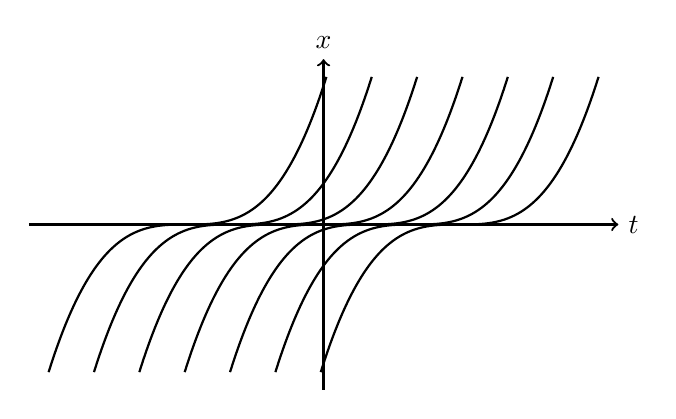
\begin{tikzpicture}[x=0.72cm,y=0.75cm,thick]
  \draw[->] (-5.2,0)--(5.2,0) node[right] {$t$};
  \draw[->] (0,-2.8)--(0,2.8) node[above] {$x$};
  \foreach \c in {-2.4,-1.6,-0.8,0,0.8,1.6,2.4} {
    \pgfmathsetmacro{\lo}{\c-2.45}
    \pgfmathsetmacro{\hi}{\c+2.45}
    \draw[domain=\lo:\hi,samples=90,smooth,variable=\t]
      plot (\t,{0.17*(\t-\c)^3});
  }
\end{tikzpicture}
}
 \caption{连续但不满足状态偏导数条件的右端使得同一初始值可对应多个解（原书图 4）。}
 \label{fig:ch1-nonunique}
\end{figure}

\section{存在和唯一性定理的叙述}

§1 讨论了一个一阶微分方程，并叙述了它的存在和唯一性定理。常微分方程理论还要处理更一般的方程组。通常，由几个一阶方程组成的系统含有几个未知函数，而这些未知函数都是同一个自变量的函数。无论方程的形式如何，存在和唯一性定理都是研究给定微分方程组的理论基础。

原书先对一种表面形式较特殊的系统叙述并证明定理；实际上，相当一般的系统都可以化成这种形式。这种特殊形式称为标准方程组。用现代列向量记号，标准系统就是
\begin{equation}
 \vect{x}'=\vect{f}(t,\vect{x}),
 \qquad
 \vect{f}:\Omega\subseteq\R\times\R^n\to\R^n.
 \label{eq:ch1-standard-system}
\end{equation}
分量形式为
\begin{equation}
 x_i'=f_i(t,x_1,\ldots,x_n),
 \qquad i=1,\ldots,n.
 \label{eq:ch1-standard-components}
\end{equation}
这里 \(t\) 是自变量，\(x_1,\ldots,x_n\) 是未知函数，而 \(f_1,\ldots,f_n\) 定义在 \(n+1\) 维空间中的开集 \(\Omega\) 上。\(\Omega\) 中点的坐标是
\[
 (t,x_1,\ldots,x_n).
\]
今后总假设 \(\vect{f}\) 在 \(\Omega\) 上连续，并且它的状态偏导数
\begin{equation}
 \frac{\partial f_i}{\partial x_j}(t,\vect{x}),
 \qquad i,j=1,\ldots,n,
 \label{eq:ch1-state-partials}
\end{equation}
在 \(\Omega\) 上存在且连续。这里强调：这些偏导数只关于 \(x_1,\ldots,x_n\) 求，不要求关于 \(t\) 的偏导数存在。

连续向量函数 \(\vect{x}:I\to\R^n\) 是系统 \eqref{eq:ch1-standard-system} 的解，是指它在 \(I\) 上可微，并且在每个 \(t\in I\) 处都有
\[
 (t,\vect{x}(t))\in\Omega,
 \qquad
 \vect{x}'(t)=\vect{f}(t,\vect{x}(t)).
\]
区间 \(I\) 称为解的定义区间，不排除 \(I=(-\infty,+\infty)\) 的情形。“在区间上满足方程组”是指把 \(x_1(t),\ldots,x_n(t)\) 代入后得到整个区间上的恒等式；因此既要求 \(\vect{x}(t)\) 在每一点可微，也要求代换后的点始终落在右端函数的定义域中。

\begin{theorem}[标准方程组的存在唯一性]
 \label{thm:ch1-system-existence}
 设 \eqref{eq:ch1-standard-system} 是标准方程组，\(\vect{f}\) 在开集 \(\Omega\subseteq\R\times\R^n\) 上有定义且连续，并且 \(D_{\vect{x}}\vect{f}\) 在 \(\Omega\) 上存在且连续。则：
 \begin{enumerate}[label=\arabic*.]
  \item 对 \(\Omega\) 中每一点 \((t_0,\vect{x}_0)\)，存在一个包含 \(t_0\) 的区间上的解 \(\vect{x}=\vect{\varphi}(t)\)，满足
  \[
   \vect{\varphi}(t_0)=\vect{x}_0.
  \]
  \item 若两个解 \(\vect{x}=\vect{\psi}(t)\) 和 \(\vect{x}=\vect{\chi}(t)\) 的定义区间都含有 \(t_0\)，并且
  \[
   \vect{\psi}(t_0)=\vect{\chi}(t_0),
  \]
  则它们在共同定义区间上处处相等。
 \end{enumerate}
\end{theorem}

证明见\hyperref[sec:existence-proofs]{本章补证}。补证在开集 \(\Omega\)、\(\vect{f}\) 连续且 \(D_{\vect{x}}\vect{f}\) 连续的条件下，用向量形式的 Picard 逐次逼近构造局部解；随后沿公共区间反复使用局部唯一性，得到整个公共区间上的唯一性；最大解一节再把所有同初值解合并成唯一的不可延拓解。

向量
\[
 \vect{x}_0=
 \begin{pmatrix}
  x_{10}\\
  \vdots\\
  x_{n0}
 \end{pmatrix}
\]
称为初始值，关系式
\begin{equation}
 \vect{x}(t_0)=\vect{x}_0
 \label{eq:ch1-initial-condition}
\end{equation}
称为初始条件。说一个解具有初始值 \(\vect{x}_0\)，总表示它的定义区间含有 \(t_0\)。定理 2 可以简述为：对任意初始值，总存在以它为初值的局部解；若两个解具有相同初值，则它们在共同定义区间上完全重合。

完全与 §1 一样，可以定义延拓和不可延拓解。设 \(\vect{x}:I\to\R^n\) 和 \(\vect{\widetilde{x}}:J\to\R^n\) 都是同一系统的解，且 \(I\subseteq J\)，\(\vect{\widetilde{x}}|_I=\vect{x}\)，则称 \(\vect{\widetilde{x}}\) 是 \(\vect{x}\) 的延拓。特别地，自身也算自身的一个延拓。若不存在任何不同于它自身、却仍以它为限制的延拓，则称该解不可延拓。在定理 2 的条件下，每一个解都可以唯一地延拓到不可延拓解；详细证明见\hyperref[sec:existence-proofs]{本章补证}中的“最大解的存在与唯一”一节。

\begin{theorem}[线性系统的整体存在性]
 \label{thm:ch1-linear-existence}
 设
 \begin{equation}
  \vect{x}'=\mat{A}(t)\vect{x}+\vect{b}(t)
  \label{eq:ch1-linear-system}
 \end{equation}
 是标准线性系统，其中
 \[
  \mat{A}:I\to\R^{n\times n},
  \qquad
  \vect{b}:I\to\R^n
 \]
 在区间 \(I=(q_1,q_2)\) 上连续。则对任意 \(t_0\in I\) 和任意 \(\vect{x}_0\in\R^n\)，系统 \eqref{eq:ch1-linear-system} 存在一个以
 \[
  \vect{x}(t_0)=\vect{x}_0
 \]
 为初始条件、并且在整个区间 \(I\) 上有定义的解。
 \end{theorem}

特别地，如果 \(\mat{A}(t)\) 和 \(\vect{b}(t)\) 在整条实轴上连续，即 \(q_1=-\infty,q_2=+\infty\)，那么对任意初值，系统都存在定义在整个无限区间 \(-\infty<t<+\infty\) 上的解。结合定理 2，整个区间上的解还是唯一的。这个结论将在\hyperref[sec:existence-proofs]{本章补证}的“线性系统为何在系数连续的整个区间上存在”一节中证明；线性迭代差的阶乘估计使逐次逼近在每个紧子区间上收敛，而不需要把时间区间缩小到压缩系数小于一。

标准系统的解有直接的几何意义。以
\[
 t,x_1,\ldots,x_n
\]
为坐标得到 \(n+1\) 维空间；解 \(\vect{x}=\vect{\varphi}(t)\) 对应于曲线
\begin{equation}
 t\longmapsto
 \begin{pmatrix}
  t\\
  \varphi_1(t)\\
  \vdots\\
  \varphi_n(t)
 \end{pmatrix}
 \in\R^{n+1}.
 \label{eq:ch1-integral-curve-system}
\end{equation}
这条曲线称为系统的积分曲线。它的切向量为
\[
 \begin{pmatrix}
  1\\
  x_1'(t)\\
  \vdots\\
  x_n'(t)
 \end{pmatrix}
 =
 \begin{pmatrix}
  1\\
  f_1(t,\vect{x}(t))\\
  \vdots\\
  f_n(t,\vect{x}(t))
 \end{pmatrix}.
\]
系统本身在 \(\Omega\) 的每一点规定了方向 \((1,\vect{f}(t,\vect{x}))\)，于是得到 \(n+1\) 维空间中的方向场。这个方向场是 §1 平面情形的高维类比。

\subsection{例题}

\paragraph{例 1：平面旋转系统.}
求解
\begin{equation}
 x_1'=-\omega x_2,
 \qquad
 x_2'=\omega x_1,
 \label{eq:ch1-rotation}
\end{equation}
其中 \(\omega\) 是实常数。集合 \(\Omega\) 是坐标 \((t,x_1,x_2)\) 的整个三维空间。直接求导可知
\begin{equation}
 x_1(t)=c_1\cos(\omega t+c_2),
 \qquad
 x_2(t)=c_1\sin(\omega t+c_2)
 \label{eq:ch1-rotation-solution}
\end{equation}
是解，其中 \(c_1,c_2\) 是常数。

要证明 \eqref{eq:ch1-rotation-solution} 包含全部解，只需证明任意初值都能由适当的常数实现。给定初值 \((t_0,x_{10},x_{20})\)，令 \((\rho,\varphi)\) 是点 \((x_{10},x_{20})\) 的极坐标，因此
\[
 x_{10}=\rho\cos\varphi,
 \qquad
 x_{20}=\rho\sin\varphi.
\]
把初值代入 \eqref{eq:ch1-rotation-solution}，得到决定 \(c_1,c_2\) 的条件
\[
 c_1\cos(\omega t_0+c_2)=x_{10},
 \qquad
 c_1\sin(\omega t_0+c_2)=x_{20}.
\]
利用极坐标化为
\[
 c_1\cos(\omega t_0+c_2)=\rho\cos\varphi,
 \qquad
 c_1\sin(\omega t_0+c_2)=\rho\sin\varphi.
\]
取
\[
 c_1=\rho,
 \qquad
 c_2=\varphi-\omega t_0,
\]
这两式便同时成立。若 \((x_{10},x_{20})=\vect{0}\)，取 \(\rho=0\) 即可。因此通过每一点 \((t_0,x_{10},x_{20})\) 都有公式 \eqref{eq:ch1-rotation-solution} 给出的解；由定理 2 的唯一性，公式包含全部解。

用矩阵写成
\[
 \vect{x}'=
 \begin{pmatrix}
  0&-\omega\\
  \omega&0
 \end{pmatrix}\vect{x},
\]
可以更直接看出右端是线性的。后文将利用复指数函数再次求解这类系统。

\paragraph{例 2：右端的光滑性与解的光滑性.}
证明：如果标准系统 \eqref{eq:ch1-standard-system} 的右端 \(\vect{f}\) 是 \(k\) 次连续可微的，也就是说 \(\vect{f}\) 对全部变量 \(t,x_1,\ldots,x_n\) 具有直到 \(k\) 阶的连续偏导数，并且包括混合偏导数，那么它的任一解 \(\vect{x}=\vect{\varphi}(t)\) 具有 \(k+1\) 阶连续导数。

事实上，对于解有恒等式
\begin{equation}
 \varphi_i'(t)=f_i(t,\varphi_1(t),\ldots,\varphi_n(t)),
 \qquad i=1,\ldots,n.
 \label{eq:ch1-solution-identity}
\end{equation}
如果 \(\vect{f}\) 具有连续的一阶偏导数，那么恒等式右端对 \(t\) 有连续导数，因此 \(\varphi_i'(t)\) 连续可微，从而 \(\varphi_i''(t)\) 存在且连续。对恒等式 \eqref{eq:ch1-solution-identity} 逐次求导，并反复使用链式法则，就可以依次证明
\[
 \varphi_i',\varphi_i'',\ldots,\varphi_i^{(k+1)}
\]
的存在性和连续性。用矩阵写出一阶导数的显式公式就是
\[
 \vect{x}''(t)
 =\vect{f}_t(t,\vect{x}(t))+D_{\vect{x}}\vect{f}(t,\vect{x}(t))\vect{x}'(t).
\]
继续求导时，还会出现 \(\vect{f}\) 的各高阶状态偏导数和混合偏导数，这正是题设要求它们连续的原因。

\section{化一般微分方程组为标准方程组}

前一节对标准方程组叙述了解的存在和唯一性定理。现在说明怎样把相当一般的高阶微分方程组化为标准方程组；同时，一般方程组的存在和唯一性结论也由此得到。

先给出一般微分方程的形式。一个未知函数 \(y\) 的方程可以写为
\begin{equation}
 F(t,y,y',\ldots,y^{(n)})=0,
 \label{eq:ch1-general-high-order}
\end{equation}
其中 \(t\) 是自变量，\(y\) 是未知函数，\(F\) 是给定的 \(n+2\) 个变量的函数。函数 \(F\) 未必对所有变量值都有定义，所以需要谈它的定义域 \(B\)，其中 \(B\) 是坐标
\[
 t,y,y',\ldots,y^{(n)}
\]
的 \(n+2\) 维空间中的开集。如果方程中导数的最高阶数等于 \(n\)，就称它是 \(n\) 阶方程。

如果定义在区间 \(r_1<t<r_2\) 上的函数 \(y=\varphi(t)\) 具有直到 \(n\) 阶的导数，使得
\[
 \bigl(t,\varphi(t),\varphi'(t),\ldots,\varphi^{(n)}(t)\bigr)\in B
\]
在整个区间上成立，并且代入后使 \eqref{eq:ch1-general-high-order} 成为恒等式，则称它是该方程的解。与一阶情形一样，必须同时检查所需导数的存在性和右端定义域。

若有同一自变量的两个未知函数 \(u,v\)，则两个微分方程组成的方程组可以写成
\begin{equation}
 \begin{cases}
  F(t,u,u',\ldots,u^{(m)},v,v',\ldots,v^{(n)})=0,\\
  G(t,u,u',\ldots,u^{(m)},v,v',\ldots,v^{(n)})=0.
 \end{cases}
 \label{eq:ch1-two-unknown-general}
\end{equation}
其中 \(F,G\) 定义在某个开集 \(B\) 上。若 \(u\) 在方程中出现的最高导数阶数为 \(m\)，\(v\) 的最高导数阶数为 \(n\)，则分别称 \(m,n\) 为方程组关于 \(u,v\) 的阶，并称
\[
 m+n
\]
为整个方程组的阶。定义在共同区间上的一对函数 \(u=\varphi(t),v=\psi(t)\) 若代入后使两个方程在整个区间上恒成立，就称为方程组的解。

对未知函数 \(y_1,\ldots,y_r\) 同样可以定义方程组。若 \(y_i\) 在方程组中出现的最高导数阶数为 \(q_i\)，则
\[
 q=q_1+\cdots+q_r
\]
称为方程组的阶。§3 的标准方程组按这种计数法是一阶方程组，因为它只含一阶导数，并且有 \(n\) 个未知函数，所以总阶数为 \(n\)。

如果关系式 \eqref{eq:ch1-general-high-order} 可以关于 \(y^{(n)}\) 解出，就得到
\begin{equation}
 y^{(n)}=f(t,y,y',\ldots,y^{(n-1)}).
 \label{eq:ch1-explicit-high-order}
\end{equation}
同样，如果两个未知函数的方程组可以关于 \(u^{(m)},v^{(n)}\) 解出，就得到
\begin{equation}
 \begin{cases}
  u^{(m)}
  =f(t,u,u',\ldots,u^{(m-1)},v,v',\ldots,v^{(n-1)}),\\
  v^{(n)}
  =g(t,u,u',\ldots,u^{(m-1)},v,v',\ldots,v^{(n-1)}).
 \end{cases}
 \label{eq:ch1-explicit-two-high-order}
\end{equation}
这两类方程称为已解出最高阶导数的方程。任意多个未知函数的方程也可以类似定义。今后几乎只研究已解出最高阶导数的系统；§3 的标准一阶系统正是其中的特殊情形。

现在证明：任何已解出最高阶导数的 \(n\) 阶微分方程组，都可以化为标准一阶方程组。先处理一个 \(n\) 阶标量方程。

\subsection{一个高阶方程的转化}

\textbf{(A) 一个 \(n\) 阶方程.} 设
\begin{equation}
 y^{(n)}=f(t,y,y',\ldots,y^{(n-1)})
 \label{eq:ch1-high-order-scalar}
\end{equation}
是一个已解出最高阶导数的 \(n\) 阶微分方程。这里 \(t\) 是自变量，\(y\) 是未知函数。函数 \(f\) 定义在 \(n+1\) 维坐标空间中的开集 \(\Gamma\) 内，其坐标是
\[
 t,y,y',\ldots,y^{(n-1)}.
\]
假设 \(f\) 在 \(\Gamma\) 上连续，并且它关于各个状态变量
\[
 y,y',\ldots,y^{(n-1)}
\]
的偏导数在 \(\Gamma\) 上也连续。这里把 \(y,y',\ldots,y^{(n-1)}\) 看成彼此独立的坐标。

为了把 \eqref{eq:ch1-high-order-scalar} 化为标准系统，引入新未知函数
\begin{equation}
 x_1=y,\qquad x_2=y',\qquad \ldots,\qquad x_n=y^{(n-1)}.
 \label{eq:ch1-companion-coordinates}
\end{equation}
把它们排成状态列向量
\begin{equation}
 \vect{x}(t)=
 \begin{pmatrix}
  x_1(t)\\
  x_2(t)\\
  \vdots\\
  x_n(t)
 \end{pmatrix}
 =
 \begin{pmatrix}
  y(t)\\
  y'(t)\\
  \vdots\\
  y^{(n-1)}(t)
 \end{pmatrix}
 \in\R^n.
 \label{eq:ch1-scalar-state}
\end{equation}
方程 \eqref{eq:ch1-high-order-scalar} 等价于标准系统
\begin{equation}
 \begin{cases}
  x_1'=x_2,\\
  x_2'=x_3,\\
  \qquad\vdots\\
  x_{n-1}'=x_n,\\
  x_n'=f(t,x_1,x_2,\ldots,x_n).
 \end{cases}
 \label{eq:ch1-companion-system}
\end{equation}
用向量形式写作
\begin{equation}
 \vect{x}'=
 \begin{pmatrix}
  x_2\\
  x_3\\
  \vdots\\
  x_n\\
  f(t,x_1,\ldots,x_n)
 \end{pmatrix}.
 \label{eq:ch1-companion-vector}
\end{equation}

下面证明“等价”在两个方向上成立。先设 \(y=\varphi(t)\) 满足 \eqref{eq:ch1-high-order-scalar}。由 \eqref{eq:ch1-companion-coordinates} 定义
\[
 x_1=\varphi,\quad x_2=\varphi',\quad\ldots,\quad x_n=\varphi^{(n-1)}.
\]
对关系式求导，得到
\begin{equation}
 x_k'=y^{(k)}=x_{k+1},
 \qquad k=1,\ldots,n-1,
 \label{eq:ch1-companion-first-equations}
\end{equation}
而
\begin{equation}
 x_n'=y^{(n)}
 =f(t,y,y',\ldots,y^{(n-1)})
 =f(t,x_1,x_2,\ldots,x_n).
 \label{eq:ch1-companion-last-equation}
\end{equation}
所以 \(\vect{x}\) 满足系统 \eqref{eq:ch1-companion-system}。

反过来，设 \(\vect{x}=(x_1,\ldots,x_n)\) 满足系统 \eqref{eq:ch1-companion-system}，并令 \(y=x_1\)。系统第一式给出
\[
 y'=x_1'=x_2.
\]
第二式给出
\[
 y''=x_2'=x_3.
\]
继续逐式代换，得到
\[
 y^{(k)}=x_{k+1},
 \qquad k=0,\ldots,n-1.
\]
最后，在系统最后一式中代入这些关系：
\[
 y^{(n)}=x_n'
 =f(t,x_1,\ldots,x_n)
 =f(t,y,y',\ldots,y^{(n-1)}).
\]
所以 \(y\) 满足原高阶方程。两段构造互相逆转，故在共同区间上，原方程的解与系统 \eqref{eq:ch1-companion-system} 的解一一对应。

原方程的初始条件通常写成
\begin{equation}
 y^{(k)}(t_0)=y_{0}^{(k)},
 \qquad k=0,1,\ldots,n-1.
 \label{eq:ch1-high-order-initial}
\end{equation}
它在变换 \eqref{eq:ch1-companion-coordinates} 下恰好变成状态初值
\begin{equation}
 \vect{x}(t_0)=
 \begin{pmatrix}
  y_0\\
  y_0'\\
  \vdots\\
  y_0^{(n-1)}
 \end{pmatrix}.
 \label{eq:ch1-state-initial}
\end{equation}
要求
\[
 (t_0,y_0,y_0',\ldots,y_0^{(n-1)})\in\Gamma.
\]
由于 \eqref{eq:ch1-companion-vector} 的右端及其 Jacobian 在相应开集上连续，定理 2 给出满足这些初始条件的局部解，并断言两个具有相同状态初值的解在共同区间上相同。

如果原方程是线性的，即
\begin{equation}
 y^{(n)}
 =a_0(t)y+a_1(t)y'+\cdots+a_{n-1}(t)y^{(n-1)}+q(t),
 \label{eq:ch1-linear-high-order}
\end{equation}
并且系数 \(a_0,\ldots,a_{n-1}\) 与自由项 \(q\) 在区间 \(I=(q_1,q_2)\) 上连续，那么系统 \eqref{eq:ch1-companion-system} 也是线性的：
\begin{equation}
 \vect{x}'=\mat{A}(t)\vect{x}+\vect{b}(t),
 \label{eq:ch1-high-order-linear-system}
\end{equation}
其中
\begin{equation}
 \mat{A}(t)=
 \begin{pmatrix}
  0&1&0&\cdots&0\\
  0&0&1&\cdots&0\\
  \vdots&\vdots&\vdots&\ddots&\vdots\\
  0&0&0&\cdots&1\\
  a_0(t)&a_1(t)&a_2(t)&\cdots&a_{n-1}(t)
 \end{pmatrix},
 \qquad
 \vect{b}(t)=
 \begin{pmatrix}
  0\\
  0\\
  \vdots\\
  0\\
  q(t)
 \end{pmatrix}.
 \label{eq:ch1-companion-linear-data}
\end{equation}
由定理 3，任意初始条件 \eqref{eq:ch1-high-order-initial} 都确定一个在整个 \(I\) 上定义的解。这就是命题 (A) 的最后一项整体存在结论。

\subsection{多个高阶方程的转化}

\textbf{(B) 两个二阶方程组成的方程组.} 为减少记号上的复杂性，原书以两个二阶方程为例：
\begin{equation}
 \begin{cases}
  u''=f(t,u,u',v,v'),\\
  v''=g(t,u,u',v,v').
 \end{cases}
 \label{eq:ch1-two-second-order}
\end{equation}
按照
\begin{equation}
 x_1=u,\qquad x_2=u',\qquad x_3=v,\qquad x_4=v'
 \label{eq:ch1-two-state-coordinates}
\end{equation}
引入新的未知函数后，方程组化成
\begin{equation}
 \begin{cases}
  x_1'=x_2,\\
  x_2'=f(t,x_1,x_2,x_3,x_4),\\
  x_3'=x_4,\\
  x_4'=g(t,x_1,x_2,x_3,x_4).
 \end{cases}
 \label{eq:ch1-two-standard-system}
\end{equation}
用列向量写就是
\begin{equation}
 \vect{x}'=
 \begin{pmatrix}
  x_2\\
  f(t,x_1,x_2,x_3,x_4)\\
  x_4\\
  g(t,x_1,x_2,x_3,x_4)
 \end{pmatrix}.
 \label{eq:ch1-two-standard-vector}
\end{equation}

假设右端函数 \(f,g\) 在五维空间中坐标为
\[
 t,u,u',v,v'
\]
的某个开集 \(\Gamma\) 上有定义且连续，并且它们关于四个状态变量的偏导数也连续，那么在 \eqref{eq:ch1-two-standard-vector} 经过坐标变换后，新的右端满足定理 2 的条件。于是对 \(\Gamma\) 中任一点
\[
 (t_0,u_0,p_0,v_0,q_0),
\]
存在满足
\begin{equation}
 u(t_0)=u_0,\qquad u'(t_0)=p_0,
 \qquad
 v(t_0)=v_0,\qquad v'(t_0)=q_0
 \label{eq:ch1-two-initial-conditions}
\end{equation}
的解 \(u=\varphi(t),v=\psi(t)\)。此外，任何两个具有同样初始条件的解，在它们定义区间的公共部分上相同。

命题 (B) 的证明与命题 (A) 完全一样。正向地，对方程组 \eqref{eq:ch1-two-second-order} 的解按 \eqref{eq:ch1-two-state-coordinates} 定义 \(x_1,\ldots,x_4\)，求导便得到系统 \eqref{eq:ch1-two-standard-system}。反向地，若 \(x_1,\ldots,x_4\) 满足该系统，令 \(u=x_1,v=x_3\)，第一式和第三式给出
\[
 u'=x_2,
 \qquad
 v'=x_4,
\]
第二式和第四式再给出原来的两个二阶方程。初始条件也在变换 \eqref{eq:ch1-two-state-coordinates} 下逐项对应。因此原方程组的解与四维标准系统的解一一对应。

对更多未知函数，做法完全相同：依次把每个未知函数和它低于最高阶的各阶导数排入状态向量。若各未知函数的最高阶数分别为 \(q_1,\ldots,q_r\)，则状态向量有
\[
 q_1+\cdots+q_r
\]
个分量。这样就把总阶数有限的已解出最高阶导数系统化成了标准一阶系统。

\subsection{尚未解出最高阶导数时的问题}

如果 \(n\) 阶方程仍以
\begin{equation}
 F(t,y,y',\ldots,y^{(n)})=0
 \label{eq:ch1-implicit-high-order}
\end{equation}
给出，而没有解出未知函数的最高阶导数 \(y^{(n)}\)，那么首先出现的问题是：能否在给定区域中解出 \(y^{(n)}\)。这更像一个函数论中的隐函数问题，但它会把一些新的现象带入微分方程研究。

例如，若 \(F\) 关于 \(y^{(n)}\) 是二次的，那么在其他变量固定时，方程可能确定 \(y^{(n)}\) 的两个值。如果这两个值在某一区域内处处不同，就可以分别研究两个形如
\[
 y^{(n)}=f_\pm(t,y,y',\ldots,y^{(n-1)})
\]
的已解出方程。但如果两个值在某个集合上重合，或不能连续地分成彼此分离的分支，就不能简单地把原方程拆成两个标准方程。研究这种情形会导致微分方程奇解的概念，以及与曲面上微分方程有关的理论。原书不讨论这些问题；本节的转化结论始终以最高阶导数已经显式解出为前提。

\subsection{例题}

\paragraph{例 1：简谐振动方程.}
求解
\begin{equation}
 y''+\omega^2y=0,
 \qquad \omega>0.
 \label{eq:ch1-harmonic}
\end{equation}
直接验证可知，函数
\begin{equation}
 y(t)=r\cos(\omega t+\alpha),
 \qquad r\ge0,
 \label{eq:ch1-harmonic-solution}
\end{equation}
满足这个方程，其中 \(r,\alpha\) 是常数。

还要证明公式 \eqref{eq:ch1-harmonic-solution} 包含全部解。设 \(y=\varphi(t)\) 是任一解。由线性高阶方程的整体存在结论，也就是命题 (A) 的末尾部分，可以认为这个解对所有 \(t\in\R\) 有定义。令
\[
 y(0)=y_0,
 \qquad
 y'(0)=v_0.
\]
直接验证可以选取常数 \(r,\alpha\)，使
\begin{equation}
 r\cos\alpha=y_0,
 \qquad
 -r\omega\sin\alpha=v_0.
 \label{eq:ch1-harmonic-initial-match}
\end{equation}
如果这些等式成立，那么公式 \eqref{eq:ch1-harmonic-solution} 给出的解与原解有相同的初始值 \((0,y_0,v_0)\)，由命题 (A) 和唯一性，它们相同。

为具体选出 \(r,\alpha\)，当 \((y_0,v_0)\neq(0,0)\) 时取
\[
 r=\sqrt{y_0^2+\frac{v_0^2}{\omega^2}},
\]
并要求
\[
 \cos\alpha=\frac{y_0}{r},
 \qquad
 \sin\alpha=-\frac{v_0}{\omega r}.
\]
两式的平方和为
\[
 \frac{y_0^2}{r^2}+\frac{v_0^2}{\omega^2r^2}=1,
\]
所以这样的 \(\alpha\) 存在；若 \(y_0=v_0=0\)，取 \(r=0\) 即可。因此公式 \eqref{eq:ch1-harmonic-solution} 确实给出全部解。

函数 \eqref{eq:ch1-harmonic-solution} 描述简谐振动。正数 \(r\) 称为振幅，\(\alpha\) 称为初相位，简称相位。方程 \eqref{eq:ch1-harmonic} 称为简谐振动方程。数 \(\omega\) 称为角频率；每单位时间内完成完整振动的次数为
\begin{equation}
 \nu=\frac{\omega}{2\pi}.
 \label{eq:ch1-frequency-harmonic}
\end{equation}
用状态 \(\vect{x}=(y,y')\) 表示，方程是
\[
 \vect{x}'=
 \begin{pmatrix}
  0&1\\
  -\omega^2&0
 \end{pmatrix}\vect{x}.
\]
两个状态分量分别是位移与速度；初值 \(\vect{x}(0)=(y_0,v_0)\) 正好同时给出这两个信息。

\paragraph{例 2：弹性回复力下的直线运动.}
讨论质量为 \(m\) 的质点 \(p\) 在力 \(F\) 的作用下沿水平直线 \(L\) 的运动。设力始终沿该直线指向固定点 \(O\)，大小与 \(p\) 到 \(O\) 的距离成正比。在直线上取 \(O\) 为原点，用 \(x=x(t)\) 表示质点 \(p\) 的有符号坐标。在物理记号中，对时间的一阶、二阶导数写为 \(\dot x,\ddot x\)。根据牛顿第二定律，
\begin{equation}
 m\ddot x=F=-kx,
 \qquad k>0.
 \label{eq:ch1-spring-newton}
\end{equation}
通常写成
\begin{equation}
 m\ddot x+kx=0.
 \label{eq:ch1-spring}
\end{equation}
负号自动处理原点两侧：当 \(x>0\) 时，力指向负方向；当 \(x<0\) 时，力指向正方向。

在物理上，这种回复力可以由弹簧实现，如图~\ref{fig:ch1-spring} 所示。数 \(k\) 称为弹簧的弹性系数。把 \eqref{eq:ch1-spring} 除以 \(m\)，与例 1 比较，得到
\begin{equation}
 x(t)=r\cos\left(\sqrt{\frac{k}{m}}\,t+\alpha\right),
 \qquad r\ge0.
 \label{eq:ch1-spring-solution}
\end{equation}
于是质点 \(p\) 的角频率
\[
 \omega=\sqrt{\frac{k}{m}}
\]
由质量 \(m\) 和弹性系数 \(k\) 决定，与初始条件无关。振幅 \(r\) 和初相位 \(\alpha\) 则与初始条件有关，也就是与 \(t=0\) 时质点 \(p\) 的位置 \(x(0)\) 和速度 \(\dot x(0)\) 有关。

\begin{figure}[H]
 \centering
 \resizebox{0.78\textwidth}{!}{\begin{tikzpicture}[x=0.8cm,y=0.8cm,thick]
  % Fixed supports and a mass between two elastic springs.
  \fill[pattern=north east lines] (-4.1,-0.58) rectangle (-3.85,0.58);
  \fill[pattern=north east lines] (3.85,-0.58) rectangle (4.1,0.58);
  \draw[thick] (-3.85,0)--(3.85,0);
  \draw[decorate,decoration={coil,aspect=0.5,segment length=4mm,amplitude=3mm}] (-3.65,0)--(-0.65,0);
  \draw[decorate,decoration={coil,aspect=0.5,segment length=4mm,amplitude=3mm}] (0.65,0)--(3.65,0);
  \draw[fill=white,thick] (0,0) circle (0.48);
  \fill (0,0) circle (1.6pt);
  \node at (0.72,0.58) {$p$};
  \draw[<->] (-0.05,0.88)--(1.45,0.88) node[midway,above] {$x$};
  \draw[->] (0,-0.72)--(-1.55,-0.72) node[midway,below] {$F$};
\end{tikzpicture}
}
 \caption{弹性回复力下的直线运动；位移 \(x\) 和回复力 \(F\) 取有符号方向（原书图 5）。}
 \label{fig:ch1-spring}
\end{figure}

\paragraph{例 3：数学摆的小振动.}
数学摆由一个质量为 \(m\) 的质点 \(p\) 组成；在重力作用下，质点沿竖直平面内半径为 \(\ell\) 的圆周 \(K\) 运动，\(\ell\) 称为摆长。取圆周最低点 \(O\) 为角坐标零点，在圆周上取正方向，用 \(\theta=\theta(t)\) 表示质点的变动角坐标，如图~\ref{fig:ch1-pendulum} 所示。为与全文三角函数记号一致，这里把原书的 \(\varphi\) 写为 \(\theta\)。

作用在质点 \(p\) 上的重力大小为 \(mg\)，方向竖直向下。重力沿圆周法线方向的分量由约束力提供的方向相反作用来平衡；重力的切向分量，若取角增加的方向为正，则等于
\[
 -mg\sin\theta.
\]
沿切线应用牛顿第二定律，质点的加速度为 \(\ell\ddot\theta\)，于是
\[
 m\ell\ddot\theta=-mg\sin\theta,
\]
或者
\begin{equation}
 \ell\ddot\theta+g\sin\theta=0.
 \label{eq:ch1-pendulum}
\end{equation}
这个方程是非线性的，求它的精确解相当困难。若在运动中角 \(\theta\) 始终与零相差很小，就可以用 \(\theta\) 代替 \(\sin\theta\)，得到摆的近似方程
\begin{equation}
 \ell\ddot\theta+g\theta=0.
 \label{eq:ch1-pendulum-linearized}
\end{equation}
它的解具有例 1 的形式：
\begin{equation}
 \theta(t)=r\cos\left(\sqrt{\frac{g}{\ell}}\,t+\alpha\right).
 \label{eq:ch1-pendulum-small-solution}
\end{equation}
因此摆的小振动角频率为
\[
 \omega=\sqrt{\frac{g}{\ell}},
\]
单位时间内完整振动次数为
\[
 \nu=\frac{\omega}{2\pi}
 =\frac{1}{2\pi}\sqrt{\frac{g}{\ell}}.
\]
例如秒摆，即每秒振动一次的摆，满足 \(\nu=1\,\mathrm{s}^{-1}\)。于是
\[
 \ell=\frac{g}{4\pi^2}\approx 0.25\,\mathrm m.
\]
这里的余弦解是小角近似方程的解，而不是非线性摆方程 \eqref{eq:ch1-pendulum} 的精确解。精确摆方程可写成标准状态系统
\[
 x_1=\theta,\quad x_2=\dot\theta,
 \qquad
 \begin{cases}
  x_1'=x_2,\\
  x_2'=-\dfrac{g}{\ell}\sin x_1.
 \end{cases}
\]

\begin{figure}[H]
 \centering
 \resizebox{0.58\textwidth}{!}{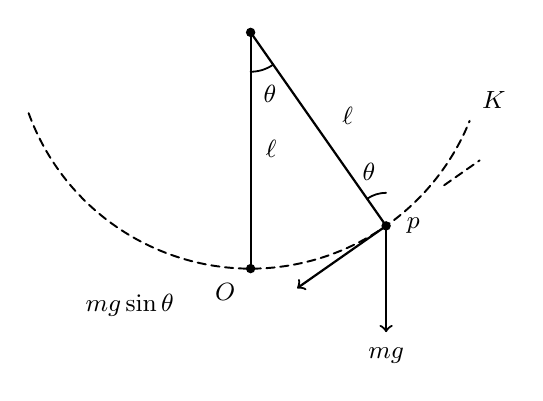
\begin{tikzpicture}[
  x=1cm,
  y=1cm,
  line cap=round,
  line join=round,
  every node/.style={font=\small}
]
  % 以悬点为圆心，O 和 p 同在半径为 l 的圆弧上。
  \def\radius{3}
  \def\swingangle{35}
  \pgfmathsetmacro{\px}{\radius*sin(\swingangle)}
  \pgfmathsetmacro{\py}{\radius-\radius*cos(\swingangle)}
  \pgfmathsetmacro{\topEndAngle}{270+\swingangle}
  \pgfmathsetmacro{\pEndAngle}{90+\swingangle}
  \pgfmathsetmacro{\pLabelAngle}{90+\swingangle/2}

  \coordinate (C) at (0,\radius);
  \coordinate (O) at (0,0);
  \coordinate (P) at (\px,\py);
  \coordinate (Kleft) at ({\radius*cos(200)},{\radius+\radius*sin(200)});
  \coordinate (Kright) at ({\radius*cos(338)},{\radius+\radius*sin(338)});
  \coordinate (TopAngleStart) at ({0.50*cos(270)},{\radius+0.50*sin(270)});
  \coordinate (TopAngleLabel) at ({0.82*cos(270+\swingangle/2)},{\radius+0.82*sin(270+\swingangle/2)});
  \coordinate (PAngleStart) at ({\px+0.42*cos(90)},{\py+0.42*sin(90)});
  \coordinate (PAngleLabel) at ({\px+0.72*cos(\pLabelAngle)},{\py+0.72*sin(\pLabelAngle)});

  % 轨道圆弧，以原图的悬点为圆心。
  \draw[densely dashed, line width=0.7pt]
    (Kleft) arc[start angle=200,end angle=338,radius=\radius cm];

  % 悬点到最低点和质点的两条半径。
  \draw[line width=0.8pt] (C)--(O);
  \draw[line width=0.8pt] (C)--(P)
    node[pos=0.56,above right=2pt] {$\ell$};
  \node[right=2pt] at (0,1.52) {$\ell$};

  % p 点处的切线及重力、切向分量。
  \pgfmathsetmacro{\tangentStartX}{\px+0.90*cos(\swingangle)}
  \pgfmathsetmacro{\tangentStartY}{\py+0.90*sin(\swingangle)}
  \pgfmathsetmacro{\tangentEndX}{\px+1.45*cos(\swingangle)}
  \pgfmathsetmacro{\tangentEndY}{\py+1.45*sin(\swingangle)}
  \pgfmathsetmacro{\componentEndX}{\px-1.38*cos(\swingangle)}
  \pgfmathsetmacro{\componentEndY}{\py-1.38*sin(\swingangle)}
  \draw[densely dashed, line width=0.7pt]
    (\tangentStartX,\tangentStartY)--(\tangentEndX,\tangentEndY);
  \draw[->,line width=0.8pt] (P)--(\px,\py-1.35)
    node[below=2pt] {$mg$};
  \draw[->,line width=0.8pt] (P)--(\componentEndX,\componentEndY);
  \node[anchor=east] at (-0.85,-0.46) {$mg\sin\theta$};

  % 两处角标相同：摆杆与竖直方向的夹角。
  \draw[line width=0.65pt] (TopAngleStart)
    arc[start angle=270,end angle=\topEndAngle,radius=0.50cm];
  \node at (TopAngleLabel) {$\theta$};
  \draw[line width=0.65pt] (PAngleStart)
    arc[start angle=90,end angle=\pEndAngle,radius=0.42cm];
  \node at (PAngleLabel) {$\theta$};

  \fill (C) circle (1.7pt);
  \fill (O) circle (1.7pt);
  \fill (P) circle (1.7pt);
  \node[below left=2pt] at (O) {$O$};
  \node[right=4pt] at (P) {$p$};
  \node[above right=1pt] at (Kright) {$K$};
\end{tikzpicture}
}
 \caption{数学摆的角坐标 $\theta$ 与重力的切向分量（据原书图 6 重绘）。}
 \label{fig:ch1-pendulum}
\end{figure}

\section{复值微分方程}

直到现在，只讨论了实值微分方程及其实解。但在某些情况下，例如求解常系数线性方程时，先求出实方程的复值解，再由复值解取得实解会更方便。为了说明这个过程，必须引入实变量的复值函数，以及复值微分方程组。

\subsection{实变量的复值函数}

\textbf{(A) 复值函数.} 如果对区间 \(r_1<t<r_2\) 上的每一个实数值 \(t\)，有复数
\begin{equation}
 z(t)=u(t)+iv(t)
 \label{eq:ch1-complex-function}
\end{equation}
与之对应，其中 \(u(t),v(t)\) 是实变量的实函数，则称 \(z\) 是实变量 \(t\) 的复值函数。函数 \(u\) 称为 \(z\) 的实部，\(v\) 称为 \(z\) 的虚部：
\[
 u(t)=\operatorname{Re}z(t),
 \qquad
 v(t)=\operatorname{Im}z(t).
\]
如果 \(u,v\) 连续，就称复值函数 \(z\) 连续；如果 \(u,v\) 可微，就称 \(z\) 可微，并定义
\begin{equation}
 z'(t)=u'(t)+iv'(t).
 \label{eq:ch1-complex-derivative}
\end{equation}
这里 \(t\) 仍然是实变量，所以这是沿实轴求导，而不是复分析意义下的全纯导数。

直接验证可知，实变量的复值函数仍满足通常的和、积、商求导法则；商法则要求分母不为零。例如
\[
 (z_1z_2)'
 =z_1'z_2+z_1z_2'.
\]
复向量值函数的连续性、可微性按每个分量定义。

\subsection{复系统的实化}

\textbf{(B) 标准复方程组.} 考虑
\begin{equation}
 \vect{z}'=\vect{h}(t,\vect{z}),
 \qquad
 \vect{z}(t)\in\C^n,
 \qquad
 \vect{h}:\Omega\subseteq\R\times\C^n\longrightarrow\C^n.
 \label{eq:ch1-complex-system}
\end{equation}
为了避免复分析中额外的可微性理论，本章按原书范围假设 \(\vect{h}\) 的每个分量都是复变量 \(z_1,\ldots,z_n\) 的多项式，并且多项式系数是实变量 \(t\) 在区间 \(I=(q_1,q_2)\) 上的连续实值或复值函数。在这个条件下，\(\vect{h}\) 对任意 \(\vect{z}\in\C^n\) 都有定义。

若定义在某个区间上的复值向量函数 \(\vect{z}(t)\) 代入 \eqref{eq:ch1-complex-system} 后得到恒等式，就称它是解。对任意 \(t_0\in I\) 和任意 \(\vect{z}_0\in\C^n\)，系统存在满足
\begin{equation}
 \vect{z}(t_0)=\vect{z}_0
 \label{eq:ch1-complex-initial}
\end{equation}
的局部解；具有相同初值的两个解在共同定义区间上相同。若系统是线性的，则解在整个 \(I\) 上有定义。

这些结论可以直接由定理 2 推出。把每个复未知函数分成实部和虚部：
\begin{equation}
 z_j=x_j+iy_j,
 \qquad j=1,\ldots,n.
 \label{eq:ch1-complex-real-components}
\end{equation}
在 \eqref{eq:ch1-complex-system} 中用 \(x_j+iy_j\) 代替 \(z_j\)，得到
\begin{equation}
 \dot x_j+i\dot y_j
 =f_j(t,x_1,\ldots,x_n,y_1,\ldots,y_n)
 +ig_j(t,x_1,\ldots,x_n,y_1,\ldots,y_n),
 \label{eq:ch1-complex-realified-component}
\end{equation}
其中 \(f_j,g_j\) 都是实变量的实值函数，并满足
\begin{equation}
 f_j+ig_j
 =h_j(t,x_1+iy_1,\ldots,x_n+iy_n).
 \label{eq:ch1-complex-real-part-definition}
\end{equation}
比较 \eqref{eq:ch1-complex-realified-component} 两边的实部和虚部，就得到实系统
\begin{equation}
 \begin{cases}
  x_j'=f_j(t,x_1,\ldots,x_n,y_1,\ldots,y_n),\\
  y_j'=g_j(t,x_1,\ldots,x_n,y_1,\ldots,y_n),
 \end{cases}
 \qquad j=1,\ldots,n.
 \label{eq:ch1-complex-realified-system}
\end{equation}
因为 \(\vect{h}\) 关于复变量是多项式，所以 \(f_j,g_j\) 关于 \(2n\) 个实变量 \(x_1,\ldots,x_n,y_1,\ldots,y_n\) 也是多项式；又因为 \(\vect{h}\) 的系数关于 \(t\) 连续，所以 \(f_j,g_j\) 的系数也关于 \(t\) 连续。于是实系统 \eqref{eq:ch1-complex-realified-system} 满足定理 2 的条件。

若
\[
 \vect{z}_0=\vect{x}_0+i\vect{y}_0,
\]
则复初始条件 \eqref{eq:ch1-complex-initial} 等价于实初始条件
\begin{equation}
 \vect{x}(t_0)=\vect{x}_0,
 \qquad
 \vect{y}(t_0)=\vect{y}_0.
 \label{eq:ch1-complex-real-initial}
\end{equation}
定理 2 给出实系统的局部存在唯一性；反过来，任何一个实系统解都可以通过 \(\vect{z}=\vect{x}+i\vect{y}\) 组成复系统解。因为两个复数相等当且仅当实部、虚部分别相等，所以这个对应在两个方向上都成立。

对线性复系统，实化可以写得很明确。设
\begin{equation}
 \vect{z}'=\mat{A}(t)\vect{z}+\vect{b}(t),
 \qquad
 \mat{A}(t)=\mat{B}(t)+i\mat{C}(t),
 \quad
 \vect{b}(t)=\vect{p}(t)+i\vect{q}(t),
 \label{eq:ch1-complex-linear}
\end{equation}
其中 \(\mat{B}(t),\mat{C}(t)\in\R^{n\times n}\)，\(\vect{p}(t),\vect{q}(t)\in\R^n\)。若 \(\vect{z}=\vect{x}+i\vect{y}\)，则
\[
 (\mat{B}+i\mat{C})(\vect{x}+i\vect{y})
 =(\mat{B}\vect{x}-\mat{C}\vect{y})+i(\mat{C}\vect{x}+\mat{B}\vect{y}).
\]
因此 \eqref{eq:ch1-complex-linear} 等价于
\begin{equation}
 \frac{\dd}{\dd t}
 \begin{pmatrix}
  \vect{x}\\\vect{y}
 \end{pmatrix}
 =
 \begin{pmatrix}
  \mat{B}(t)&-\mat{C}(t)\\
  \mat{C}(t)&\mat{B}(t)
 \end{pmatrix}
 \begin{pmatrix}
  \vect{x}\\\vect{y}
 \end{pmatrix}
 +
 \begin{pmatrix}
  \vect{p}(t)\\\vect{q}(t)
 \end{pmatrix}.
 \label{eq:ch1-complex-linear-realified}
\end{equation}
这是 \(2n\) 维实线性系统，系数连续，因此由定理 3，解在整个 \(I\) 上存在。矩阵 \eqref{eq:ch1-complex-linear-realified} 中的四个块顺序不能随意调换：左上、右下分别来自 \(\mat{A}\) 的实部和虚部，右上块带负号，左下块带正号。

最后指出，右端为复变量多项式的复系统，其多项式系数可能全部是 \(t\) 的实函数。即使如此，仍可把 \(z_1,\ldots,z_n\) 看成复变量并寻找复值解。这样做是因为某些实系统求复值解比直接求实值解更容易。先求复值解，再从中分出实值解；所谓分出，就是只保留虚部恒为零的那些复值解。对一般非线性方程，不能把任意复值解的实部直接当作实值解。

\subsection{高阶复方程}

\textbf{(C) \(n\) 阶复方程.} 设
\begin{equation}
 z^{(n)}
 =f(t,z,z',\ldots,z^{(n-1)})
 \label{eq:ch1-complex-high-order}
\end{equation}
是 \(n\) 阶复值方程。假设右端是关于复变量
\[
 z,z',\ldots,z^{(n-1)}
\]
的多项式，其系数是实变量 \(t\) 在 \(I=(q_1,q_2)\) 上的实值或复值连续函数。如果
\[
 t_0\in I,
\]
而 \(z_0,z_0',\ldots,z_0^{(n-1)}\) 是任意复数，那么方程 \eqref{eq:ch1-complex-high-order} 存在满足
\begin{equation}
 z(t_0)=z_0,
 \quad
 z'(t_0)=z_0',
 \quad
 \ldots,
 \quad
 z^{(n-1)}(t_0)=z_0^{(n-1)}
 \label{eq:ch1-complex-high-order-initial}
\end{equation}
的局部复值解。任何两个具有相同初始条件的解，在定义区间的公共部分上相同。若方程是线性的，即右端多项式关于各状态变量是一次多项式，则对任意初始值，解都在整个 \(I\) 上有定义。

证明与 §4 命题 (A) 相同。令
\begin{equation}
 \vect{\zeta}=
 \begin{pmatrix}
  z\\z'\\\vdots\\z^{(n-1)}
 \end{pmatrix}
 \in\C^n.
 \label{eq:ch1-complex-state}
\end{equation}
原方程等价于复标准系统
\begin{equation}
 \vect{\zeta}'=
 \begin{pmatrix}
  \zeta_2\\
  \zeta_3\\
  \vdots\\
  \zeta_n\\
  f(t,\zeta_1,\ldots,\zeta_n)
 \end{pmatrix}.
 \label{eq:ch1-complex-companion}
\end{equation}
正向地，若 \(z\) 满足高阶方程，按 \eqref{eq:ch1-complex-state} 定义状态向量，逐分量求导即得系统。反向地，令 \(z=\zeta_1\)；系统前 \(n-1\) 式依次给出
\[
 \zeta_{k+1}=z^{(k)},
 \ k=0,\ldots,n-1,
\]
最后一式给出原高阶方程。新的右端是复变量的多项式，因此前面复系统实化的存在唯一性结论适用；线性高阶方程产生线性复系统，整体存在性由定理 3 的复值版本得到。

\subsection{复指数函数}

\textbf{(D) \(e^w\) 的定义与性质.} 令 \(w=u+iv\) 是任意复数，定义
\begin{equation}
 e^w=e^u(\cos v+i\sin v).
 \label{eq:ch1-complex-exponential-definition}
\end{equation}
由此容易看出
\begin{equation}
 e^{\overline w}=\overline{e^w}.
 \label{eq:ch1-complex-conjugate-exponential}
\end{equation}
下面证明乘法公式
\begin{equation}
 e^{w_1}e^{w_2}=e^{w_1+w_2}.
 \label{eq:ch1-complex-exponential-product}
\end{equation}
由此可直接取得 Euler 公式：
\begin{equation}
 \cos v=\frac{e^{iv}+e^{-iv}}2,
 \qquad
 \sin v=\frac{e^{iv}-e^{-iv}}{2i}.
 \label{eq:ch1-euler-formulas}
\end{equation}
若 \(\lambda=\mu+i\nu\) 是复数，则根据定义
\begin{equation}
 e^{\lambda t}
 =e^{\mu t}
 \bigl(\cos(\nu t)+i\sin(\nu t)\bigr).
 \label{eq:ch1-exponential-real-time}
\end{equation}

也可以用幂级数
\begin{equation}
 e^w=1+w+\frac{w^2}{2!}+\frac{w^3}{3!}+\cdots
 \label{eq:ch1-complex-exponential-series}
\end{equation}
定义 \(e^w\)，再证明它与 \eqref{eq:ch1-complex-exponential-definition} 相同。原书把三角函数定义式 \eqref{eq:ch1-complex-exponential-definition} 作为出发点，本稿沿用这一安排。

现在证明乘法公式。设
\[
 w_1=u_1+iv_1,
 \qquad
 w_2=u_2+iv_2.
\]
由定义和三角函数和角公式，
\[
 \begin{aligned}
 e^{w_1}e^{w_2}
 &=e^{u_1}(\cos v_1+i\sin v_1)
   e^{u_2}(\cos v_2+i\sin v_2)\\
 &=e^{u_1+u_2}
   \bigl(\cos(v_1+v_2)+i\sin(v_1+v_2)\bigr)\\
 &=e^{w_1+w_2}.
 \end{aligned}
\]
特别地，由 \(e^{iv}e^{-iv}=1\) 和上述乘法公式即可得到 \eqref{eq:ch1-euler-formulas}。

再证明关于实时间 \(t\) 的求导公式
\begin{equation}
 \frac{\dd}{\dd t}e^{\lambda t}
 =\lambda e^{\lambda t}.
 \label{eq:ch1-complex-exponential-derivative}
\end{equation}
先讨论纯虚数 \(\lambda=iv\) 的情形：
\[
 \begin{aligned}
 \frac{\dd}{\dd t}e^{ivt}
 &=\frac{\dd}{\dd t}\bigl(\cos vt+i\sin vt\bigr)\\
 &=-v\sin vt+iv\cos vt\\
 &=iv(\cos vt+i\sin vt)
 =iv e^{ivt}.
 \end{aligned}
\]
对于任意 \(\lambda=\mu+i\nu\)，由
\[
 e^{\lambda t}=e^{\mu t}e^{i\nu t}
\]
和乘积求导法则，得到
\[
 \begin{aligned}
 \frac{\dd}{\dd t}e^{\lambda t}
 &=
 \left(\frac{\dd}{\dd t}e^{\mu t}\right)e^{i\nu t}
 +e^{\mu t}\frac{\dd}{\dd t}e^{i\nu t}\\
 &=\mu e^{\mu t}e^{i\nu t}
 +i\nu e^{\mu t}e^{i\nu t}
 =(\mu+i\nu)e^{\lambda t}
 =\lambda e^{\lambda t}.
 \end{aligned}
\]

\subsection{复值方程例题}

\paragraph{例 1：复指数解与二维实系统.}
讨论复方程
\begin{equation}
 z'=\lambda z,
 \qquad
 z=x+iy,
 \qquad
 \lambda=\mu+i\nu,
 \label{eq:ch1-complex-linear-example}
\end{equation}
其中 \(z\) 是实变量 \(t\) 的复值未知函数。由公式 \eqref{eq:ch1-complex-exponential-derivative}，对任意复常数 \(c\)，
\begin{equation}
 z(t)=ce^{\lambda t}
 \label{eq:ch1-complex-exponential-solution}
\end{equation}
都是 \eqref{eq:ch1-complex-linear-example} 的解。

要证明 \eqref{eq:ch1-complex-exponential-solution} 包含全部解，可以像 §1 例 1 那样使用唯一性；这里改用定理 3，以便稍微简化计算。由于方程是线性复方程，可以认为任一解对所有实数值 \(t\) 都有定义。设任一解为 \(z=\chi(t)\)，令 \(z(0)=z_0\)。在 \eqref{eq:ch1-complex-exponential-solution} 中取 \(c=z_0\)，得到
\[
 z=z_0e^{\lambda t},
\]
它与 \(\chi(t)\) 具有相同的初始值 \((0,z_0)\)。由唯一性，两者相同。因此全部解都由 \eqref{eq:ch1-complex-exponential-solution} 给出。

若 \(c=re^{i\alpha}\)，其中 \(r>0\)、\(\alpha\in\R\)，则非零解可以写成
\begin{equation}
 z(t)=re^{\lambda t+i\alpha}.
 \label{eq:ch1-complex-polar-solution}
\end{equation}
若 \(c=0\)，取 \(r=0\) 即可。把 \eqref{eq:ch1-complex-linear-example} 分成实部和虚部：
\[
 x'+iy'=(\mu+i\nu)(x+iy)
 =(\mu x-\nu y)+i(\nu x+\mu y).
\]
于是
\begin{equation}
 \begin{cases}
  x'=\mu x-\nu y,\\
  y'=\nu x+\mu y.
 \end{cases}
 \label{eq:ch1-complex-real-system-example}
\end{equation}
两个实方程的方程组 \eqref{eq:ch1-complex-real-system-example} 等价于一个复方程 \eqref{eq:ch1-complex-linear-example}。再把 \eqref{eq:ch1-complex-polar-solution} 展开：
\[
 \begin{aligned}
 x(t)+iy(t)
 &=re^{\mu t}
 \bigl(\cos(\nu t+\alpha)+i\sin(\nu t+\alpha)\bigr),
 \end{aligned}
\]
因此
\begin{equation}
 \begin{cases}
  x(t)=re^{\mu t}\cos(\nu t+\alpha),\\
  y(t)=re^{\mu t}\sin(\nu t+\alpha).
 \end{cases}
 \label{eq:ch1-complex-real-solution-example}
\end{equation}
用复数乘法求出的实系统解 \eqref{eq:ch1-complex-real-solution-example}，正是复方法的价值所在。写成矩阵就是
\[
 \frac{\dd}{\dd t}
 \begin{pmatrix}
  x\\y
 \end{pmatrix}
 =
 \begin{pmatrix}
  \mu&-\nu\\
  \nu&\mu
 \end{pmatrix}
 \begin{pmatrix}
  x\\y
 \end{pmatrix}.
\]

\paragraph{例 2：非线性复方程的实化.}
设
\begin{equation}
 z'=z^2+iz,
 \qquad
 z=x+iy,
 \label{eq:ch1-nonlinear-complex-example}
\end{equation}
其中 \(z\) 是实变量 \(t\) 的复值未知函数。把右端展开：
\[
 (x+iy)^2+i(x+iy)
 =x^2-y^2+2ixy+ix-y
 =x^2-y^2-y+i(2xy+x).
\]
比较实部和虚部，原复方程等价于
\begin{equation}
 \begin{cases}
  x'=x^2-y^2-y,\\
  y'=2xy+x.
 \end{cases}
 \label{eq:ch1-nonlinear-complex-real-system}
\end{equation}
这个例子说明，即使不求解，也可以通过实化把一个复方程化为两个实方程。

\section{线性微分方程的基本性质}

如果在微分方程组中出现的所有未知函数以及它们的导数都是一次的，那么就称这个方程组是线性的。因此，线性微分方程组的一般形式可以写成
\begin{equation}
 \sum_{j,k}a_{ijk}(t)(x_j)^{(k)}+b_i(t)=0,
 \qquad i=1,\ldots,n.
 \label{eq:ch1-linear-general-components}
\end{equation}
这里 \(x_1,\ldots,x_n\) 是自变量 \(t\) 的未知函数，系数 \(a_{ijk}(t)\) 和自由项 \(b_i(t)\) 都是 \(t\) 的函数。若所有自由项恒等于零，就称方程组为齐次的。从每一个线性方程组中丢掉自由项，就得到与它对应的齐次方程组：
\begin{equation}
 \sum_{j,k}a_{ijk}(t)(x_j)^{(k)}=0,
 \qquad i=1,\ldots,n.
 \label{eq:ch1-linear-homogeneous-components}
\end{equation}

下面的性质都假设所有系数和自由项在共同区间
\[
 I=(q_1,q_2)
\]
上有定义且连续，所讨论的解都在整个 \(I\) 上给定。为了用矩阵书写，令出现的最高导数阶数为 \(N\)，并把没有出现的项系数补为零。定义
\begin{equation}
 \mat{A}_k(t)=\bigl(a_{ijk}(t)\bigr)_{i,j=1}^{n},
 \qquad
 k=0,\ldots,N,
 \label{eq:ch1-linear-coefficient-matrices}
\end{equation}
以及
\begin{equation}
 \vect{b}(t)=
 \begin{pmatrix}
  b_1(t)\\
  \vdots\\
  b_n(t)
 \end{pmatrix},
 \qquad
 \vect{x}^{(0)}(t)=\vect{x}(t).
 \label{eq:ch1-linear-forcing-vector}
\end{equation}
那么 \eqref{eq:ch1-linear-general-components} 可以写成
\begin{equation}
 \sum_{k=0}^{N}\mat{A}_k(t)\vect{x}^{(k)}(t)+\vect{b}(t)=\vect{0}.
 \label{eq:ch1-linear-matrix-general}
\end{equation}
定义线性微分算子
\begin{equation}
 L[\vect{x}](t)=\sum_{k=0}^{N}\mat{A}_k(t)\vect{x}^{(k)}(t).
 \label{eq:ch1-linear-operator}
\end{equation}
于是非齐次方程是
\begin{equation}
 L[\vect{x}]+\vect{b}=\vect{0},
 \label{eq:ch1-linear-operator-equation}
\end{equation}
而对应的齐次方程是
\begin{equation}
 L[\vect{x}]=\vect{0}.
 \label{eq:ch1-linear-operator-homogeneous}
\end{equation}
这里没有假设最高阶系数矩阵 \(\mat{A}_N(t)\) 可逆；下面的性质只依赖 \(L\) 的线性性。

对任意常数 \(\alpha,\beta\) 和充分光滑的函数 \(\vect{u},\vect{v}\)，有
\begin{equation}
 L[\alpha \vect{u}+\beta \vect{v}]
 =\alpha L[\vect{u}]+\beta L[\vect{v}].
 \label{eq:ch1-linear-operator-linearity}
\end{equation}
事实上，
\[
 \begin{aligned}
 L[\alpha \vect{u}+\beta \vect{v}](t)
 &=\sum_{k=0}^{N}\mat{A}_k(t)
  \bigl(\alpha \vect{u}^{(k)}(t)+\beta \vect{v}^{(k)}(t)\bigr)\\
 &=\alpha\sum_{k=0}^{N}\mat{A}_k(t)\vect{u}^{(k)}(t)
  +\beta\sum_{k=0}^{N}\mat{A}_k(t)\vect{v}^{(k)}(t)\\
 &=\alpha L[\vect{u}](t)+\beta L[\vect{v}](t).
 \end{aligned}
\]

\subsection{齐次解可以线性组合}

\textbf{(A) 齐次解的性质.} 如果
\[
 \vect{x}=\vect{\varphi}(t),
 \qquad
 \vect{x}=\vect{\psi}(t)
\]
都是线性齐次方程组 \eqref{eq:ch1-linear-operator-homogeneous} 的解，而 \(c_1,c_2\) 是两个任意常数，那么
\begin{equation}
 \vect{x}(t)=c_1\vect{\varphi}(t)+c_2\vect{\psi}(t)
 \label{eq:ch1-homogeneous-combination}
\end{equation}
也是齐次方程组的解。对三个以及更多个齐次解，类似结论成立。

证明只需使用线性性：
\[
 L[c_1\vect{\varphi}+c_2\vect{\psi}]
 =c_1L[\vect{\varphi}]+c_2L[\vect{\psi}]
 =c_1\cdot\vect{0}+c_2\cdot\vect{0}=\vect{0}.
\]
因此齐次解集合在相加和数乘下封闭，是函数空间中的向量子空间：
\[
 \ker L
 =
 \{\vect{x}:L[\vect{x}]=\vect{0}\}.
\]
这里相加和数乘的对象都是整条函数，例如
\[
 (c_1\vect{\varphi}+c_2\vect{\psi})(t)
 =c_1\vect{\varphi}(t)+c_2\vect{\psi}(t).
\]

\subsection{非齐次解之差与特解加齐次解}

\textbf{(B) 两个非齐次解之差.} 设
\[
 \vect{x}=\vect{\psi}(t),
 \qquad
 \vect{x}=\vect{\chi}(t)
\]
都是非齐次方程组
\[
 L[\vect{x}]+\vect{b}=\vect{0}
\]
的解。那么
\begin{equation}
 \vect{y}(t)=\vect{\chi}(t)-\vect{\psi}(t)
 \label{eq:ch1-difference-of-solutions}
\end{equation}
是齐次方程组 \(L[\vect{y}]=\vect{0}\) 的解，因为
\[
 L[\vect{\chi}-\vect{\psi}]=L[\vect{\chi}]-L[\vect{\psi}]=(-\vect{b})-(-\vect{b})=\vect{0}.
\]

其次，如果
\[
 \vect{y}=\vect{\varphi}(t)
\]
是齐次方程组的解，而
\[
 \vect{x}=\vect{\psi}(t)
\]
是非齐次方程组 \eqref{eq:ch1-linear-operator-equation} 的解，那么
\begin{equation}
 \vect{x}(t)=\vect{\varphi}(t)+\vect{\psi}(t)
 \label{eq:ch1-particular-plus-homogeneous}
\end{equation}
仍是非齐次方程组的解。确实，
\[
 L[\vect{\varphi}+\vect{\psi}]+\vect{b}
 =L[\vect{\varphi}]+L[\vect{\psi}]+\vect{b}
 =\vect{0}+(-\vect{b})+\vect{b}=\vect{0}.
\]

两句话合在一起说明：只要非齐次方程有一个特解 \(\vect{\psi}\)，它的全部解就是
\begin{equation}
 \{\vect{\psi}(t)+\vect{y}(t):L[\vect{y}]=\vect{0}\}
 =\vect{\psi}+\ker L.
 \label{eq:ch1-affine-solution-set}
\end{equation}
这是原书性质 (B) 的现代集合表述。\(\vect{x}=\vect{\psi}\) 不是唯一的；选不同的特解，只会把整个齐次解子空间平移。这里没有断言 \(\vect{\psi}+\ker L\) 的维数，因为一般形式 \eqref{eq:ch1-linear-matrix-general} 尚未假设最高阶系数矩阵可逆。

\subsection{自由项的线性叠加}

\textbf{(C) 自由项可以分拆.} 设线性方程组的自由项具有和的形式
\begin{equation}
 b_i(t)=\alpha c_i(t)+\beta d_i(t),
 \qquad i=1,\ldots,n,
 \label{eq:ch1-forcing-decomposition}
\end{equation}
其中 \(\alpha,\beta\) 是常数。写成列向量就是
\[
 \vect{b}(t)=\alpha \vect{c}(t)+\beta \vect{d}(t).
\]
除了原方程组
\begin{equation}
 L[\vect{x}]+\alpha \vect{c}+\beta \vect{d}=\vect{0}
 \label{eq:ch1-superposition-target}
\end{equation}
以外，再考虑两个辅助方程组
\begin{equation}
 L[\vect{x}]+\vect{c}(t)=\vect{0},
 \label{eq:ch1-superposition-first}
\end{equation}
和
\begin{equation}
 L[\vect{x}]+\vect{d}(t)=\vect{0}.
 \label{eq:ch1-superposition-second}
\end{equation}
如果
\begin{equation}
 \vect{x}=\vect{\varphi}(t)
 \label{eq:ch1-superposition-first-solution}
\end{equation}
是 \eqref{eq:ch1-superposition-first} 的解，而
\begin{equation}
 \vect{x}=\vect{\chi}(t)
 \label{eq:ch1-superposition-second-solution}
\end{equation}
是 \eqref{eq:ch1-superposition-second} 的解，那么
\begin{equation}
 \vect{x}(t)=\alpha\vect{\varphi}(t)+\beta\vect{\chi}(t)
 \label{eq:ch1-superposition-combination}
\end{equation}
是原方程组 \eqref{eq:ch1-superposition-target} 的解。

证明为
\[
 \begin{aligned}
 L[\alpha\vect{\varphi}+\beta\vect{\chi}]+\alpha \vect{c}+\beta \vect{d}
 &=\alpha L[\vect{\varphi}]+\beta L[\vect{\chi}]+\alpha \vect{c}+\beta \vect{d}\\
 &=\alpha(-\vect{c})+\beta(-\vect{d})+\alpha \vect{c}+\beta \vect{d}\\
 &=\vect{0}.
 \end{aligned}
\]
因此，可以把自由项拆成若干部分，分别求出对应方程的解，再按与自由项相同的系数组合。它与 (A) 中“齐次解可以任意线性组合”是同一个线性原则的两个不同用法：组合自由项时，必须同时组合对应的解；只改变解而不相应改变自由项，一般得不到原方程的解。
